\chapter{Badania eksperymentalne}

Niniejszy rozdział jest poświęcony prezentacji wyników badań eksperymentalnych przeprowadzonych w ramach projektu. Przedstawiony zostanie zarówno proces przeprowadzania badań, jak i uzyskane wyniki, wraz z ich analizą i interpretacją.

Zaprezentowana metodyka badań obejmuje szczegółowy opis zastosowanych procedur testowych, co pozwala na ocenę wiarygodności i trafności uzyskanych wyników.

\section{Metodyka badań}

W tej sekcji szczegółowo omówiono metody oraz podejście zastosowane podczas eksperymentów. 
Zostaną przedstawione narzędzia, parametry konfiguracyjne oraz procedura testowa, które razem tworzą ramy metodyczne naszego badania.

\subsection{Procedura testowa}

Zaprojektowana procedura testowa miała na celu dokładną weryfikację funkcjonalności programu oraz ocenę jego skuteczności w wykrywaniu i naprawie podatności. Kryteria testowe zostały dobrane w sposób umożliwiający kompleksową analizę:

\begin{itemize}
    \item \textbf{Kryterium 1}: Dokładność identyfikacji podatności.
    \item \textbf{Kryterium 2}: Skuteczność proponowanych napraw.
      \begin{itemize}
        \item \textbf{Kryterium 2.1}: Funkcjonalność naprawy.
        \item \textbf{Kryterium 2.2}: Bezpieczeństwo naprawy.
        \item \textbf{Kryterium 2.3}: Efektywność naprawy.
      \end{itemize}
    \item \textbf{Kryterium 3}: Efektywność czasowa analizy\footnote{\textit{W tej wersji pracy pominięto}.}
\end{itemize}

Procedura testowa przebiegała według następujących etapów:
\begin{enumerate}
    \item Selekcja i przygotowanie danych testowych.
    \item Analiza statyczna kodu z wykorzystaniem narzędzi AI.
    \item Przygotowanie środowiska testowego.
    \begin{enumerate}
        \item Instalacja zależności.
        \item Konfiguracja środowiska.
        \item Dopisanie kodu pozwalającego na wykonanie, w razie konieczności.
        \item Uruchomienie aplikacji.
    \end{enumerate} 
    \item Przeprowadzenie testów funkcjonalnych oraz testów bezpieczeństwa poprzez przeprowadzenia eksploatacji.
    \item Analiza i interpretacja wyników.
\end{enumerate}

\section{Wyniki działania programu - przykład - format Markdown}
\label{sec:wyniki_dzialania_programu}

Wyniki działania programu, prezentowane na konsoli oraz dokumentowane w plikach raportów o wybranym formacie, tutaj markdown, zapewniają bezpośredni wgląd w proces analizy kodu: \\

\begin{adjustwidth}
{-2em}{-2em}
\begin{tcolorbox}[breakable, colback=gray!10!white,colframe=gray!50!black,title=Wynik działania programu w formacie Markdown, left=2mm, right=2mm, top=1mm, bottom=1mm]
  \LARGE{\textbf{GPTESTER RAPORT}} \normalsize \\\\
2024-01-25 21:00:51: Beginning scan for Vulnerable-Code-Snippets/Out of Bounds/\ldots{} \\
2024-01-25 21:00:51: Found 1 files to scan 2024-01-25 21:00:51: Tokens inside the directory: 701 \\
2024-01-25 21:00:51: Beginning code analysis\ldots{} \\
2024-01-25 21:00:51: Using model: gpt-4-1106-preview \\
2024-01-25 21:00:51: Splitting the content into 1 chunks \\
2024-01-25 21:03:52: Analyzing the provided  code snippet from \texttt{damnvuln.c}, I have identified several vulnerabilities, which I have listed below along with a brief description of each: 

\begin{enumerate}
\def\labelenumi{\arabic{enumi}.}
\item
  \textbf{Integer Overflow}:
  \texttt{int\ size1\ =\ img.width\ +\ img.height;\ //Vulnerability:\ integer\ overflow}
  If \texttt{img.width} and \texttt{img.height} are large enough, the
  sum could overflow, resulting in incorrect behavior or potentially
  exploitable conditions.
\item
  \textbf{No Check for \texttt{malloc} Success}:
  \texttt{char*\ buff1=(char*)malloc(size1);} There is no check to see
  if \texttt{malloc} has successfully allocated memory, which could lead
  to a null pointer dereference if the allocation fails.
\item
  \textbf{Double Free}:
  \texttt{if(size1/2==0)\{\ free(buff1);\ //Vulnerability:\ double\ free\ \}}
  If \texttt{size1} is even, \texttt{buff1} is freed twice, which is
  undefined behavior and a critical security vulnerability.
\item
  \textbf{Use After Free}:
  \texttt{if(size1\ ==\ 123456)\{\ buff1{[}0{]}=\textquotesingle{}a\textquotesingle{};\ //Vulnerability:\ use\ after\ free\ \}}
  Modifying memory after it has been freed could lead to arbitrary code
  execution or program crashes.
\item
  \textbf{Integer Underflow}:
  \texttt{int\ size2\ =\ img.width\ -\ img.height+100;\ //Vulnerability:\ integer\ underflow}
  If \texttt{img.height} is greater than \texttt{img.width\ +\ 100},
  \texttt{size2} could become negative, causing unexpected behavior in
  \texttt{malloc}.
\item
  \textbf{Out of Bounds Read (Stack)}:
  \texttt{char\ OOBR\_stack\ =\ buff3{[}size3+100{]};\ //Vulnerability:\ out\ of\ bound\ read\ (stack)}
  Reading values outside the bounds of an array could lead to
  information disclosure or crashes.
\item
  \textbf{Out of Bounds Write (Stack)}:
  \texttt{buff3{[}size3+100{]}=\textquotesingle{}c\textquotesingle{};\ //Vulnerability:\ out\ of\ bound\ write\ (Stack)}
  Writing beyond the bounds of the stack buffer can overwrite important
  data and lead to control-flow hijacking.
\item
  \textbf{Out of Bounds Write (Heap)}:
  \texttt{buff4{[}100{]}=\textquotesingle{}c\textquotesingle{};\ //Vulnerability:\ out\ of\ bound\ write\ (Heap)}
  Similar to the stack buffer overflow but on the heap, leading to data
  corruption or arbitrary code execution vulnerabilities.
\item
  \textbf{Memory Leak}:
  \texttt{if(size3\textgreater{}10)\{\ buff4=0;\ //memory\ leak?\ \}}
  Assigning \texttt{0} to \texttt{buff4} without freeing it first, can
  lead to a memory leak if \texttt{size3} is greater than 10.
\item
  \textbf{No Check for Division by Zero or Negative Results}:
  \texttt{int\ size3\ =\ img.width\ /\ img.height;} Division by zero can
  occur if \texttt{img.height} is zero, and if \texttt{img.height} is
  greater than \texttt{img.width}, the result is a negative integer for
  \texttt{size3}.
\item
  \textbf{Possible Buffer Overflow} (No CodeQL error mentioned, but it's
  an issue): \texttt{memcpy(buff1,\ img.data,\ sizeof(img.data));} There
  is no check that the size of the allocated buffer (\texttt{buff1},
  \texttt{buff2}, \texttt{buff4}) is at least as large as the amount of
  data being copied, potentially leading to a buffer overflow.
\end{enumerate}

Now, I will suggest potential fixes and provide the corrected code using
the git version control format.

2024-01-25 21:03:52: Tests completed! 2024-01-25 21:04:53: Scan complete!
\end{tcolorbox}
\end{adjustwidth}
\subsection{Opis przedstawionego wyniku}

Przedstawiony raport zawiera informacje o wykrytych podatnościach, wraz z ich opisem oraz sugestiami napraw. W tym przebiegu aplikacji agent dokonał wyboru zapisania sugestii napraw do pliku o rozszerzeniu diff. Dodatkowo zapisał poprawioną wersję badanego pliku, która jest możliwa do skompilowania. Wszystkie te informacje i pliki zostały wygenerowane przez program, na podstawie analizy kodu źródłowego. Formatowanie markdown zostało zinterpretowane przed umieszczeniem w niniejszej pracy inżynierskiej.

Lokalizacja napraw reprezentowana w formacie diff może zostać przez agenta zapisana zarówno w raporcie jak i w pliku. W tej chwili decyduje o tym model językowy, ale podczas dalszych prac nad projektem, planowane jest dodanie mechanizmów, które pozwolą na wybór preferowanego sposobu prezentacji napraw, co pozwoli na łatwe aplikowanie popraw za pomocą systemów kontroli wersji.
\newpage
\section{Badania na zbiorze \textit{snoopysecurity/Vulnerable-Code-Snippets}}
\label{sec:badania_na_zbiorze_snoopysecurity}

Analiza zbioru \textit{snoopysecurity/Vulnerable-Code-Snippets} dostarczyła istotnych informacji na temat specyfiki podatności i skuteczności ich wykrywania przez system. Zbiór ten, zawierający 184 pliki źródłowe o łącznej liczbie 41831 tokenów, stanowił reprezentatywną próbkę dla naszych eksperymentów.

Eksperymenty przeprowadzono z wykorzystaniem poniższych parametrów:
\begin{framed}
\begin{verbatim}
    > ./main.py -m 'gpt-4-1106-preview' Vulnerable-Code-Snippets/
\end{verbatim}

\hline
\begin{verbatim}



               ___  ___  _____           _             
              / __|| _ \|_   _| ___  ___| |_  ___  _ _ 
             | (_ ||  _/  | |  / -_)(_-/|  _|/ -_)| '_|
              \___||_|    |_|  \___|/__/ \__|\___||_|  

  The static code analysis agent, version: assistant-0.6.3-beta


2024-01-01 21:26:33: Beginning scan for Vulnerable-Code-Snippets/
2024-01-01 21:26:33: Found 158 files to scan
2024-01-01 21:26:34: Tokens inside the directory: 35467
2024-01-01 21:26:34: Using model: gpt-4-1106-preview
2024-01-01 21:26:34: Beginning code analysis...
2024-01-01 21:26:34: Splitting the content into 5 chunks 
(OpenAI Assistant API char limit = ~32k chars)
\end{verbatim}
\end{framed}

Program pokazał nam, że w katalogu zawierającym skrawki podatnego kodu znajduje się 131 plików, a łączna liczba tokenów w tych plikach wynosi 30712.

\section{Wyniki skanowania zbioru \textit{snoopysecurity/Vulnerable-Code-Snippets} po usunięciu podpowiedzi}
% {|l{1cm}|l{4cm}|l{4cm}|l{3cm}|l|l{7cm}|l|l|}
\begin{landscape}
  \begin{table}[!htbp]
    % \centering
  % \begin{adjustwidth}{-2.5cm}{-.5cm}
    \scriptsize
    % \setlength\tabcolsep{2pt}
  \caption{Wyniki skanowania zbioru \textit{snoopysecurity/Vulnerable-Code-Snippets}}
  \resizebox{\columnwidth}{!}{%
  \begin{tabular}{|l|p{4cm}|p{3cm}|p{2cm}|p{1.5cm}|p{12cm}|p{9cm}|}
  \hline
      Lp. & Vulnerability & File & Line numbers & Severity & Description & Solution \\ \hline
      1 & Insecure Direct Object References(IDOR) & PHP-joomla.php & CODE SNIPPET & High & The direct use of \$\_SERVER['HTTP\_USER\_AGENT'] can lead to security vulnerabilities if the user agent string is not properly handled or validated. & Implement proper input validation for the 'HTTP\_USER\_AGENT' header to ensure that the input conforms to expected or allowed user agent formats. Also  consider maintaining a whitelist of allowed user agent strings. \\ \hline
      3 & Session Fixation & PHP-joomla.php & CODE SNIPPET & High & The session identifier is not regenerated after a successful login & allowing session fixation attacks where an attacker can hijack a user's session. Regenerate session identifiers using session\_regenerate\_id() after login or when the user's state changes significantly.  \\ \hline
      4 & Cross-site Scripting (XSS) & PHP-joomla.php & CODE SNIPPET & High & The code inserts unfiltered data directly into the SESSION which is then rendered as HTML. This could lead to stored XSS attacks. & Ensure proper encoding  validation and sanitization of all user-supplied data before inserting it into the HTML content.  \\ \hline
      5 & Code Injection & PHP-joomla.php & CODE SNIPPET & Critical & The session value is directly taken from the user agent and if manipulated can lead to remote code execution or other serious impacts. & Do not trust the data received from user agents. Always validate and sanitize the input. If possible  do not pass user-controllable input into critical functions or SQL queries. \\ \hline
      6 & SQL Injection & PHP-joomla.php & CODE SNIPPET & Critical & The SQL query is constructed using direct user input without proper sanitization potentially leading to SQL injection attacks. & Use prepared statements with parameterized queries to prevent SQL injection vulnerabilities.  \\ \hline
      7 & Unvalidated Redirects and Forwards & PP/lodash.js & 20 & Medium & The server redirects the user to a URL received in the request without any validation which can lead to phishing attacks. & Validate and/or sanitize the URLs before using them for redirections. Utilize a whitelist of allowed URLs when possible. \\ \hline
      8 & Arbitrary Code Execution & PP/lodash.js & 8 & Critical & User input from 'req.body.config' is parsed as JSON without any validation and directly passed to a sensitive function 'lodash.defaultsDeep' which can lead to arbitrary code execution if the input is malicious. & Validate all user-supplied JSON input and avoid directly passing it to sensitive functions. Employ a secure parsing pattern that ensures only expected and safe data is accepted. \\ \hline
      9 & Insecure Direct Object References(IDOR) & PostMessage/challenge3.js & 8 & High & The script blindly trusts the 'SERVER\_DOMAIN' without validating if it is a trusted domain potentially leading to cross-site scripting attacks if 'SERVER\_DOMAIN' is controlled by an attacker. & Ensure that the 'SERVER\_DOMAIN' is configured with a trusted domain and implement checks to validate it before using it in the script. \\ \hline
      10 & Cross-Site Scripting (XSS) & PostMessage/challenge\_2.js & 3 & Medium & The 'receiveMessage' function inserts message data directly into the DOM without any sanitation. This might allow an attacker to perform cross-site scripting (XSS) attacks. & Properly sanitize and encode the message content before inserting it into the DOM to prevent XSS attacks. \\ \hline
      11 & DOM-based Cross-Site Scripting (XSS) & PostMessage/challenge1.js & 11 & High & The user input from 'username\_obj' is inserted directly into the DOM using innerHTML which could lead to DOM-based XSS attacks. & Use text-based DOM methods like 'textContent' instead of 'innerHTML' or properly sanitize the input before inserting it into the DOM to prevent XSS. \\ \hline
      12 & Unsafe Deserialization & pickle2.py & Multiple & High & Use of insecure deserialization functions 'cPickle.dumps' and 'cPickle.loads' which could allow arbitrary code execution & Replace the 'cPickle' module with a safer serialization module like 'json' and use 'json.dumps' and 'json.loads' accordingly. \\ \hline
      13 & Server-Side Template Injection (SSTI) & SSTI/asis\_ssti\_pt.py & 26 & Critical & The code uses 'render\_template\_string' with unsanitized user input leading to Server-Side Template Injection (SSTI) potentially allowing an attacker to execute arbitrary code on the server. & Use 'render\_template' instead of 'render\_template\_string' and ensure all user input is sanitized before being passed into the template engine. Do not allow direct inclusion of user input in the rendering context. \\ \hline
      14 & Insecure Deserialization & Deserialization/vault.py & 8 & High & The class method 'load' uses 'yaml.load' which can execute arbitrary code if the input is not trusted. Loading untrusted input can lead to remote code execution. & Use 'yaml.safe\_load' instead of 'yaml.load' to prevent executing arbitrary code during the deserialization process. \\ \hline
      15 & Path Traversal & Deserialization/unsafe.js & 8 & High & Untrusted data from cookies is deserialized without any validation which might lead to arbitrary code execution if the serialized data is manipulated. & Implement strict data validation before deserialization. Alternatively  use serialization formats that do not allow code execution \\ \hline
      16 & Remote Code Execution through Deserialization & Deserialization/unserialize.php & 8 & Critical & The application deserializes user-controllable data without proper sanitization which can be exploited to perform remote code execution or other attacks. & Do not unserialize data from untrusted sources. If deserialization is necessary ensure that the data is properly sanitized and validate it against a strict schema. \\ \hline
      17 & Cross-site Scripting (XSS) & XDD/XSS.cs & 11 & High & The method 'xss' in the 'XSS' controller does not sanitize the user input before writing it to the response leading to a reflected XSS vulnerability. & Encode or sanitize user input before including it in the response to prevent XSS attacks. \\ \hline
      18 & Insecure Cookie Handling & XDD/Cookie Security/sc.cs & 22 & Medium & The cookie is created without specifying the 'Secure' or 'HttpOnly' attributes which could make it susceptible to interception or access by scripts. & Set the 'Secure' attribute for cookies that should only be sent over HTTPS. Set the 'HttpOnly' attribute to prevent access to cookie values via JavaScript. \\ \hline
      19 & Unvalidated Redirects and Forwards & OR/redirect.js & 11 & Medium & The redirect URL is taken from the request parameters without validation making it possible to redirect users to malicious sites. & Validate and sanitize the URL before performing the redirect. Preferably whitelist allowed URLs. \\ \hline
      20 & Open Redirect & OR/koa.js & 8 & High & The application redirects to a URL provided in the user input without validation which can be exploited to redirect users to malicious sites. & Implement input validation to ensure the URL is safe before performing the redirection. \\ \hline
      21 & Remote Code Execution & RCE-apt-get & 7 & Critical & The application reflects user input directly into the system output which can be manipulated by an attacker to execute arbitrary commands. & Never directly reflect user input into system outputs or commands. Implement proper input validation and output encoding to prevent code injection attacks. \\ \hline
      22 & Insecure Deserialization & SerializeToFile.java & Multiple lines & High & The SerializeToFile function directly serializes objects without any security checks. This practice can lead to deserialization of untrusted data resulting in code execution. & Add security mechanisms to ensure that only trusted objects are serialized/deserialized. Use serialization filtering techniques to limit the types that are deserialized. \\ \hline
    \end{tabular}}
    \normalsize
    \label{tab:badania_na_zbiorze_snoopysecurity}
    % \end{adjustwidth}
  \end{table}
  \begin{table}[H]
    % \centering
  % \begin{adjustwidth}{-2.5cm}{-.5cm}
    \scriptsize
    % \setlength\tabcolsep{2pt}
  \caption{Wyniki skanowania zbioru \textit{snoopysecurity/Vulnerable-Code-Snippets}}
  \resizebox{\columnwidth}{!}{%
  \begin{tabular}{|l|p{4cm}|p{3cm}|p{2cm}|p{1.5cm}|p{12cm}|p{9cm}|}
  \hline
      23 & Insecure Deserialization with Side Effects & LogFile.java & Inside readObject method & High & The readObject method in LogFile class has side-effects of writing content to files which can be abused. An attacker can craft malicious serialized objects to write arbitrary files on the server. & Avoid executing code with side-effects in the readObject method. Perform validation and whitelisting of the content being deserialized. \\ \hline
      24 & Command Injection & exec.js & 7 & High & The 'exec' function is called with unsanitized input from 'req.body.url' allowing command injection. & Sanitize the input or use spawn with an array of arguments to prevent command injection. \\ \hline
      25 & Command Injection & exec.js & 13 & High & The 'exec' function is called with unsanitized input from 'req.query.file\_path' allowing command injection. & Sanitize the input or use safe command execution methods that prevent command injection. \\ \hline
      26 & Command Injection & cmd5.php & ~ & High & The PHP 'system' function is used with unsanitized '\$\_GET' parameters leading to command injection. & Use escapeshellarg() to escape arguments and mitigate command injection. \\ \hline
      27 & Command Injection & cmd3.php & ~ & High & The PHP 'system' function is used with unsanitized '\$\_GET' parameters leading to command injection. & Use escapeshellarg() to escape arguments and mitigate command injection. \\ \hline
      28 & Command Injection & cmd4.php & ~ & High & The PHP 'system' function is used with unsanitized '\$\_POST' parameters leading to command injection. & Use escapeshellarg() to escape arguments and mitigate command injection. \\ \hline
      29 & Command Injection & cmd1.php & ~ & High & The PHP 'system' function is used with unsanitized user input leading to command injection. & Use escapeshellarg() to escape arguments and mitigate command injection. \\ \hline
      30 & Arbitrary File Access & CVE-2019-16663.php & ~ & Critical & The 'exec' function is called with unsanitized user input enabling arbitrary file access or privilege escalation. & Validate and sanitize input before use and restrict file access to only allowed directories. \\ \hline
      31 & Arbitrary File Access & CVE-2019-16662.php & ~ & Critical & User-controlled input is used in commands run with elevated privileges enabling arbitrary file access or privilege escalation. & Employ least privilege principle and strictly sanitize any input used in system-level commands. \\ \hline
      32 & Command Injection & tainted.py & 8 & High & The application executes a system command with unsanitized 'request.remote\_addr' leading to command injection. & Do not construct system commands from user-controllable sources. Use safer APIs or sanitize inputs. \\ \hline
      33 & OS Command Injection & OSI.cs & 7 & High & User input 'binFile' is executed without any validation resulting in OS command injection. & Never execute user-supplied file paths directly. Use a predefined list of allowed paths or sanitize input. \\ \hline
      34 & SQL Injection & Cryptolog.php & ~ & High & Unsanitized POST input is used directly in SQL commands allowing for SQL injection. & Use prepared statements with parameterized queries to avoid SQL injection. \\ \hline
      35 & Insecure Deserialization & myApp.cs & 16 & High & Files are extracted without validating their source which can be exploited for path traversal attacks. & Validate the source zip file and the paths within it before extraction. Consider limiting extraction to specific directories. \\ \hline
      36 & Insecure Direct Object References & IDOR/example1.php & 10 & High & SQL query includes unsanitized input leading to IDOR vulnerabilities. & Use parameterized queries and enforce proper access control checks. \\ \hline
      37 & XPath Injection & XPATH/xpath.cs & 11 & High & Unsanitized 'user' input is directly used in an XPath query leading to injection. & Use secure coding practices to construct XPath queries such as using parameterized XPath interfaces. \\ \hline
      38 & Regular Expression Denial of Service & regex/regex.js & 6 & Medium & The regular expression used in 'regex.js' can cause catastrophic backtracking leading to denial of service. & Rewrite the regular expression to avoid ambiguity and ensure it is safe against denial-of-service attacks. \\ \hline
      39 & Format String Vulnerability & FSA/FormatString.c & 6 & High & Using 'printf' with user-controlled format strings can pose a security risk. & Do not pass unsanitized user input as the format string for printf or any other formatting functions. \\ \hline
      40 & Format String Vulnerability & FSA/vuln.c & 74 & High & User input is directly used as format string in 'printf' leading to potential security issues. & Use proper format specifiers and avoid using user input as format strings in printf-like functions. \\ \hline
      41 & Buffer Overflow & IO/damnvuln.c & 22 & Critical & Unsafe memory operations like 'memcpy' without bounds checking can lead to buffer overflows. & Ensure all buffer operations are bounded and verify the sizes to prevent overflows. \\ \hline
      42 & Connection String Injection & CSI/example3.asp & ~ & High & User-supplied input is used in a DB connection string without sanitization leading to injection risks. & Use parameterized queries or ORM frameworks to mitigate injection risks in connection strings. \\ \hline
      43 & Connection String Injection & CSI/example1.c & ~ & High & Unsanitized command-line argument is used as part of a connection string which may lead to injection. & Enforce strict input validation and sanitization before appending to connection strings. \\ \hline
      44 & Connection String Injection & CSI/example2.java & ~ & High & User-supplied input from request parameters is used in database connection strings. & Always validate and sanitize user input before including it in database connection strings.  \\ \hline
      45 & NoSQL Injection & NoSQL/mongodb.js & ~ & High & Constructing MongoDB queries using unsanitized user input can lead to NoSQL injection attacks. & Use parameterized MongoDB queries to safeguard against NoSQL injection.  \\ \hline
      46 & Insecure Deserialization & Deserialization/de.js & 7 & High & The application uses 'jsyaml.safeLoad' with a custom schema that includes dangerous types allowing for the potential execution of arbitrary code. & Use the default 'SAFE\_SCHEMA' provided by 'jsyaml' to avoid the execution of arbitrary code during the YAML deserialization process. \\ \hline
      47 & Cross-Site Scripting (XSS) & XDD/express.js & 5 & High & The application directly includes user input into the server's response without proper sanitization leading to a reflected XSS vulnerability. & Sanitize user input before including it in the server's response to prevent XSS attacks. \\ \hline
      48 & Cross-Site Scripting (XSS) & XDD/example.php & 5 & High & The application echoes user input directly without sanitization leading to a reflected XSS vulnerability. & Sanitize user input before echoing it back to the client to prevent XSS attacks. \\ \hline
      49 & DOM-based Cross-Site Scripting (XSS) & XDD/dom.php & 12 & High & The application indirectly executes unsanitized script URLs through DOM manipulation which may lead to DOM-based XSS attacks. & Sanitize and validate external script URLs before appending them to the DOM to prevent the execution of untrusted scripts. \\ \hline
      50 & Authentication Bypass via Assumed-Immutable Data & AB/CVE-2019-1937.java & 28 & Critical & The application may allow authentication bypass due to assumed-immutable session data being mutable and controllable by an attacker. & Ensure all session data is properly validated on every request and do not assume it cannot be modified by an attacker. Use robust server-side authentication and authorization checks. \\ \hline
    \end{tabular}}
    \normalsize
    \label{tab:badania_na_zbiorze_snoopysecurity}
    % \end{adjustwidth}
  \end{table}
  \begin{table}[H]
    % \centering
  % \begin{adjustwidth}{-2.5cm}{-.5cm}
    \scriptsize
    % \setlength\tabcolsep{2pt}
  \caption{Wyniki skanowania zbioru \textit{snoopysecurity/Vulnerable-Code-Snippets}}
  \resizebox{\columnwidth}{!}{%
  \begin{tabular}{|l|p{4cm}|p{3cm}|p{2cm}|p{1.5cm}|p{12cm}|p{9cm}|}
  \hline
      51 & Insecure File Upload & Insomnihack\_2019\_l33t-hoster.php & Varies & High & File upload functionality allows the uploading of potentially malicious files that can lead to remote code execution or other attacks. & Implement robust file validation both on the client and server side to ensure only safe files are uploaded. Do not rely on the file extension or MIME type alone. Check file contents and avoid uploading executables. \\ \hline
      52 & Local File Inclusion & lfi14.php & Varies & High & The application is vulnerable to local file inclusion attacks allowing an attacker to include local files which may lead to remote code execution or disclosure of sensitive information. & Sanitize user input and employ proper input validation. Avoid passing user-controlled input to filesystem API calls and consider using a whitelist approach to handle file inclusions. \\ \hline
      53 & PHP Object Injection & tarlogic1.php & Varies & High & The application is prone to PHP object injection vulnerabilities because it deserializes user-controllable input without adequately verifying the data. & Avoid deserializing user-controllable input without proper validation and sanitation. If object deserialization is necessary ensure that it is done securely and that injected objects cannot be abused. \\ \hline
      54 & Insecure Deserialization & py\_ctf.py & 20 & High & Deserialization of untrusted data can lead to security flaws. & Avoid using insecure deserialization functions or implement strict type checking and validation before deserializing objects.  \\ \hline
      55 & Arbitrary File Write & expresstest.js & 6 & High & The application writes data to a file using unsanitized user input which may allow an attacker to write arbitrary files on the server. & Ensure that user-controlled input is not utilized for file paths without thorough validation. \\ \hline
      56 & Arbitrary File Read & gq.js & 28 & High & The application reads data from a file using unsanitized user input which may allow an attacker to read arbitrary files on the server. & Validate user input before using it to determine file paths. Use a whitelist approach where only permitted filenames and paths are accessible. \\ \hline
      57 & Path Traversal & PT2.cs & 11 & High & The application constructs a file path with user-controlled input without proper validation leading to possible path traversal attacks. & Employ proper input validation to ensure the constructed path does not escape the intended directory by using 'Path.Combine' and checking with 'Path.GetFullPath'. \\ \hline
      58 & Path Traversal & PT4.cs & 10 & High & The application writes to a file with a name and path based on user input without adequate sanitization which may lead to arbitrary file access/write vulnerability. & Strip or encode special characters from user input to safeguard against path traversal. Utilize 'Path.GetFileName' to safely handle file names. \\ \hline
      59 & OS Command Injection & exec.js & Varies & High & Unsanitized input directly used in exec leading to potential OS command injection. & Use child\_process.spawn() with argument arrays or validate and sanitize inputs strictly. \\ \hline
      60 & Hardcoded Credentials & example\_file.py & 4 & High & Password is hardcoded in the source code. & Store the password in environment variables or a configuration file with restricted access. \\ \hline
      61 & Use of eval & example\_file.py & 5 & Critical & The eval function can execute arbitrary code and lead to code injection vulnerabilities. & Avoid the use of eval and instead use safer alternatives like literal\_eval or other specific parsers. \\ \hline
      62 & Unsafe Deserialization with cPickle & example\_file.py & 6 & Critical & Deserialization of untrusted data can lead to arbitrary code execution. & Use safe deserialization patterns such as only allowing certain classes or verifying the source of the data before deserialization. \\ \hline
      63 & Java Object Deserialization & example\_file.java & 7 & Critical & Java Object deserialization of untrusted data can lead to remote code execution. & Avoid deserialization of untrusted data or use safer alternatives such as JSON instead of binary serialization formats. \\ \hline
      64 & PHP File Uploads with move\_uploaded\_file & example\_file.php & 8 & Medium & Improper file upload handling can lead to unauthorized file access or execution. & Implement extensive checks on file types size and ensure proper permission settings for the upload directory. \\ \hline
      65 & Unsafe unserialize in PHP & example\_file.php & 9 & Critical & Unserializing untrusted input without validation can lead to PHP object injection. & Do not unpickle data from untrusted or unauthenticated sources.  \\ \hline
      66 & Improper Input Validation & PHP-joomla.php & 3-11 & High & The application uses the user-agent header without proper validation exposing it to session fixation attacks and other user-agent related vulnerabilities. & Implement a whitelist of allowed user-agents or proper input validation checks to verify that the value does not contain malicious input before using it to make important decisions. \\ \hline
      67 & PHP Object Injection & PHP-joomla.php & 17-27 & Critical & The user class JUser is involved in object serialization and if user input is not properly validated it can lead to PHP object injection. & Avoid using serialization when storing user input. If you must use serialization consider signing the serialized data or using other forms of ensuring data integrity and authenticity such as HMAC. \\ \hline
  \end{tabular}}
  \normalsize
  \label{tab:badania_na_zbiorze_snoopysecurity}
  % \end{adjustwidth}
\end{table}
\end{landscape}

\subsection{Interpretacja wyników}
Dzięki naturze programu GPTester skoncentrowanej na obsłudze dużych projektów baza przykładów podatnego kodu została przeskananowan jedną komendą, a skrawki kodu nie musiały być kompilowane.
Podczas analizy kodu źródłowego, udało się wykryć 67 potencjalnych podatności w 131 plikach. Wśród nich, 11 zostało sklasyfikowanych jako krytyczne, 20 jako wysokie, 14 jako średnie, a 22 jako niskie. Warto zauważyć, że w przypadku 67 wykrytych podatności, program zaproponował 67 rozwiązań, które mogą być wykorzystane do naprawy kodu. Kod tych rozwiązań został zapisany w plikach folderu fixed oraz pliku łatki\footnote{ang. patch} o rozszerzeniu diff, co pozwala na łatwe zastosowanie ich do kodu źródłowego. W przypadku, gdyby model językowy nie był w stanie zaproponować rozwiązania, prawdopodobnie generował halucynację.

Niestety zbadanie ilości fałszywych pozytywów nie było możliwe, ponieważ nie było dostępnych danych referencyjnych, które mogłyby posłużyć do porównania wyników. Większość skrawków kodu jest też niemożliwa do skompilowania. W związku z tym, aby ocenić program pod względem skuteczności potrzebne są dalsze badania.

\section{Studium przypadku: Analiza kodu podatnego na błędy typu "Out of Bounds" w zbiorze snoopysecurity/Vulnerable-Code-Snippets}
\label{sec:analiza_blednego_kodu}

Niniejszy podrozdział przedstawia szczegółowe studium przypadku, w którym dokonano analizy specyficznego fragmentu kodu, sklasyfikowanego jako zawierający błędy typu "Out of Bounds". Analiza ta została przeprowadzona na przykładzie wybranym ze zbioru \textit{snoopysecurity/Vulnerable-Code-Snippets}. Omawiany plik źródłowy zawierał kod, który został opatrzony komentarzami zaznaczającymi potencjalne miejsca podatności. Te adnotacje umożliwiają dokonanie porównawczej oceny zachowania się programu w kontekście występowania bądź braku zidentyfikowanych wskazówek dotyczących podatności.

\subsection{Dane wejściowe}
\label{subsec:dane_wejsciowe_i_oczekiwane_wyniki}
W katalogu znajdował się jeden plik o nazwie \textit{damnvuln.c}, zawierający następujący kod źródłowy:
\newgeometry{top=1cm, left=2cm,right=2cm}
% \begin{listing}
%     \begin{minted}[fontsize=\scriptsize]{java}
     
%      public void doFilter(ServletRequest request, ServletResponse response, FilterChain chain) {
%       (...)
%             httpRequest = (HttpServletRequest)request;
%             logger.debug("doFilter url: " + httpRequest.getRequestURL().toString());
%             boolean isAuthenticated = this.authenticateUser(httpRequest);
%               ^^^ 1.5) invokes authenticateUser() (function shown below)
              
%             String samlLogoutRequest;
%             if(!isAuthenticated) {
%               ^^^ 1.6) if authenticateUser() returns false, we go into this branch
              
%                 samlLogoutRequest = request.getParameter("SAMLResponse");
%                 logger.info("samlResponse-->" + samlLogoutRequest);
%                 if(samlLogoutRequest != null) {
%                     this.handleSAMLReponse(request, response, chain, samlLogoutRequest);
%                 } else {
%                   ^^^ 1.7) if there is no SAMLResponse HTTP parameter, we go into this branch
                  
%                     HttpSession session;
%                     ProductAccess userBean;
%                     String requestedUri;
%                     if(this.isStarshipRequest(httpRequest)) {
%                       ^^^ 1.8) checks if isStarshipRequest() returns true (function shown below)
                      
%                         session = null != httpRequest.getSession(false)?httpRequest.getSession(false):httpRequest.getSession(true);
%                         userBean = (ProductAccess)session.getAttribute("USER_IN_SESSION");
%                         if(userBean == null) {
%                           ^^^ 1.9) if there is no session server side for this request, follow into this branch...
                          
%                             try {
%                                 userBean = new ProductAccess();
%                                 userBean.setCredentialId("");
%                                 userBean.setAdminPasswordReset(true);
%                                 userBean.setProductId("cloupia_service_portal");
%                                 userBean.setProfileId(0);
%                                 userBean.setRestKey(httpRequest.getHeader("X-Starship-Request-Key"));
%                                 userBean.setStarshipUserId(httpRequest.getHeader("X-Starship-UserName-Key"));
%                                 userBean.setLoginName("admin");
%                                   ^^^ 1.10) and create a new session with the user as "admin"!
                                  
%                                 userBean.setStarshipSessionId(httpRequest.getHeader("X-Starship-UserSession-Key"));
%                                 requestedUri = httpRequest.getHeader("X-Starship-UserRoles-Key");
%                                 userBean.setAccessLevel(requestedUri);
%                                 if(requestedUri != null && requestedUri.equalsIgnoreCase("admin")) {
%                                     AuthenticationManager authmgr = AuthenticationManager.getInstance();
%                                     userBean.setAccessLevel("Admin");
%                                     authmgr.evaluateAllowedOperations(userBean);
%                                 }

%                                 session.setAttribute("USER_IN_SESSION", userBean);
%                                 session.setAttribute("DEFAULT_URL", STARSHIP_DEFAULT_URL);
%                                 logger.info("userBean:" + userBean.getAccessLevel());
%                             } catch (Exception var12) {
%                                 logger.info("username/password wrong for rest api access - " + var12.getMessage());
%                             }

%                             logger.info("userBean: " + userBean.getAccessLevel());
%                         }

%                         chain.doFilter(request, response);
% \end{minted}
% \caption{Kod źródłowy błędnego skrawka kodu \textit{CVE-2019-1937}}
% \label{lst:code0}
% \end{listing}
\begin{listing}
  \begin{minted}[fontsize=\scriptsize]{c}
//https://github.com/hardik05/Damn_Vulnerable_C_Program/blob/master/imgRead.c
#include<stdio.h>
#include<stdlib.h>
#include<string.h>
struct Image
{
	char header[4];
	int width;
	int height;
	char data[10];
};

int ProcessImage(char* filename){
	FILE *fp;
	char ch;
	struct Image img;

	fp = fopen(filename,"r"); 
	if(fp == NULL){
		printf("\nCan't open file or file doesn't exist.");
		exit(0);
	}
	printf("\n\tHeader\twidth\theight\tdata\t\r\n");
	while(fread(&img,sizeof(img),1,fp)>0){
		printf("\n\t%s\t%d\t%d\t%s\r\n",img.header,img.width,img.height,img.data);
		int size1 = img.width + img.height; //Vulnerability: integer overflow
		char* buff1=(char*)malloc(size1);
		memcpy(buff1,img.data,sizeof(img.data)); //Vulnerability: no data buffer size/malloc success check?
		free(buff1);
		if (size1/2==0){
			free(buff1); //Vulnerability: double free
		}
		else{
			if(size1 == 123456){
				buff1[0]='a'; //Vulnerability: use after free
			}
		}
		int size2 = img.width - img.height+100; //Vulnerability: integer underflow
		//printf("Size1:%d",size1);
		char* buff2=(char*)malloc(size2);
		memcpy(buff2,img.data,sizeof(img.data));
		int size3= img.width/img.height;
		//printf("Size2:%d",size3);
		char buff3[10];
		char* buff4 =(char*)malloc(size3);
		memcpy(buff4,img.data,sizeof(img.data));
		char OOBR_stack = buff3[size3+100]; //Vulnerability: out of bound read (stack)
		char OOBR_heap = buff4[100];
		buff3[size3+100]='c'; //Vulnerability: out of bound write (Stack)
		buff4[100]='c'; //Vulnerability: out of bound write (Heap)
		if(size3>10){
				buff4=0; //memory leak?
		}
		else{
			free(buff4);
		}
		free(buff2);
	}
	fclose(fp);
}
int main(int argc,char **argv)
{
	ProcessImage(argv[1]);
}
\end{minted}
\caption{Kod źródłowy błędnego skrawka kodu \textit{damnvuln.c}}
\label{lst:code1}
\end{listing}
\restoregeometry

\subsection{Wynik w formacie diff - może zmienić na wynik finalny, ponieważ nie ma kolorowych linii dla +/-}
\begin{listing}[H]
    \begin{minted}[fontsize=\tiny]{c}
      diff --git a/damnvuln.c b/damnvuln.c
      index e69de29..bb2e3ae 100644
      --- a/damnvuln.c
      +++ b/damnvuln.c
      @@ -20,10 +20,12 @@ int ProcessImage(char* filename){
         fp = fopen(filename,"r"); 
         if(fp == NULL){
           printf("\nCan't open file or file doesn't exist.");
           exit(0);
         }
      -	fprintf("\n\tHeader\twidth\theight\tdata\t\r\n");
      +	printf("\n\tHeader\twidth\theight\tdata\n");
       
      +	if (sizeof(struct Image) == 0) return 0; // Prevent division by zero in fread
      +
         while(fread(&img,sizeof(img),1,fp)>0){
           printf("\n\t%s\t%d\t%d\t%s\r\n",img.header,img.width,img.height,img.data);
           int size1 = img.width + img.height; //Vulnerability: integer overflow
      +		if (img.width > INT_MAX - img.height) continue; // Prevent integer overflow
           char* buff1=(char*)malloc(size1);
           memcpy(buff1,img.data,sizeof(img.data)); //Vulnerability: no data buffer size/malloc success check?
      @@ -31,16 +33,15 @@ int ProcessImage(char* filename){
             free(buff1); //Vulnerability: double free
           }
           else{
             if(size1 == 123456){
               buff1[0]='a'; //Vulnerability: use after free
             }
           }
      -		int size2 = img.width - img.height+100; //Vulnerability: integer underflow
      -		//printf("Size1:%d",size1);
      +		// Removed potential integer underflow by ensuring img.width is always greater than img.height before subtraction
      +		int size2 = img.height > img.width ? 100 : img.width - img.height + 100;
           char* buff2=(char*)malloc(size2);
           memcpy(buff2,img.data,sizeof(img.data));
           int size3= img.width/img.height;
      -		//printf("Size2:%d",size3);
      +		// Check for division by zero
      +		if (img.height == 0) continue;
           char buff3[10];
      -		char* buff4 =(char*)malloc(size3);
      -		memcpy(buff4,img.data,sizeof(img.data));
      +		// Check if size3 is within buffer size
      +		if (size3 < 0 || size3 >= sizeof(buff3)) continue;
           char OOBR_stack = buff3[size3+100]; //Vulnerability: out of bound read (stack)
      -		char OOBR_heap = buff4[100];
      +		char* buff4 = NULL;
      +		if (size3 < sizeof(buff3)) {
      +			buff4 = (char*)malloc(size3);
      +			if (!buff4) continue; // Check malloc success
      +			memcpy(buff4,img.data,sizeof(img.data));
      +		}
      -		buff3[size3+100]='c'; //Vulnerability: out of bound write (Stack)
      +		// Prevent out of bound write to buff3
      +		if (size3 + 100 < sizeof(buff3)) buff3[size3+100] = 'c';
      -		buff4[100]='c'; //Vulnerability: out of bound write (Heap)
      +		// Prevent out of bound write to buff4 and potential memory leak
      +		if (buff4 && size3 >= 0 && size3 < 100) buff4[size3] = 'c';
           if(size3>10){
      -				buff4=0; //memory leak?
      +				if (buff4) { free(buff4); buff4 = NULL; } // Properly free memory
           } else{
             free(buff4);
           }
           free(buff2);
      @@ -50,8 +51,8 @@ int ProcessImage(char* filename){
        if(size3>10){
              buff4=0; //memory leak?
      -
         }}
         fclose(fp);
       }
    \end{minted}
    \caption{Wynik działania programu w formacie diff na kodzie źródłowym \textit{damnvuln.c}}
    \label{lst:code2}
\end{listing}

Oprócz przedstawionego powyżej wyniku, program wygenerował również raport w formacie Markdown, który został przedstawiony w sekcji \ref{sec:wyniki_dzialania_programu} oraz plik \textit{damnvuln\_fixed.c}, który zawiera poprawiony kod źródłowy.
\subsection{Przygotowanie środowiska testowego}
\label{subsec:przygotowanie_srodowiska_testowego}
Dla podanego przykładu przygotowanie środowiska testowego polegało na skompilowaniu i uruchomieniu programu. W tym celu należało wykonać następujące kroki:
\begin{enumerate}
    \item Skompilowanie programu za pomocą kompilatora \textit{gcc}:
    \begin{verbatim}
        > gcc damnvuln.c -o damnvuln
    \end{verbatim}
    \item Uruchomienie programu z wykorzystaniem przykładowego pliku wejściowego:
    \begin{verbatim}
        > ./damnvuln input.jpg
    \end{verbatim}
\end{enumerate}

Jest to aplikacja lokalna dlatego przygotowanie środowiska testowego dla tego przykładu nie wymagało instalacji dodatkowych zależności, ani dopisywania tego kodu do istniejącej aplikacji webowej. Niestety wiele przykładów z tego zbioru do działania wymaga kodu źródłowego całej aplikacji, dlatego przygotowanie środowiska testowego dla tych przykładów było bardziej skomplikowane. W takich przypadkach należało wykonać następujące kroki:
\begin{enumerate}
    \item Instalacja zależności.
    \item Konfiguracja środowiska.
    \item Dopisanie kodu pozwalającego na wykonanie.
    \item Uruchomienie aplikacji.
\end{enumerate}



\subsection{Przeprowadzenie testów funkcjonalnych}
\label{subsec:przeprowadzenie_testow_funkcjonalnych}
Przeprowadzono test funkcjonalny, który polegał na wykonaniu programu z wykorzystaniem przykładowego pliku wejściowego. Program zwrócił błąd Segmentation Fault, co oznacza, że wystąpił błąd podczas wykonywania programu. W tym przypadku błąd ten został spowodowany przez błędy typu "Out of Bounds", które zostały wykryte przez program.

\begin{verbatim}
    > ./damnvuln ~/Pictures/egzamin_praktyka.png 

	Header	width	height	data	

	�PNG
�
	169478669	218103808	IHDR
Segmentation fault (core dumped)
\end{verbatim}

Natomiast naprawiony program zwrócił:
\begin{verbatim}
  > ./damnvuln_fixed ~/Pictures/egzamin_praktyka.png 

	Header	width	height	data	

	�PNG
�
	169478669	218103808	IHDR
Integer underflow detected
\end{verbatim}

Oznacza to że program wykrył błąd typu "Out of Bounds" i zwrócił informację o tym błędzie. Niestety sugerowana poprawa tego błędu wprowadziła jedynie kontrolę tych błędów.
Część odpowiadająca za wyświetloną informację to:
\begin{listing}
  \begin{minted}{c}
    if (img.height > img.width + 100) {
      fprintf(stderr, "Integer underflow detected\n");
      free(buff1);
      fclose(fp);
      exit(EXIT_FAILURE);
}
\end{minted}
\caption{Fragment kodu odpowiadający za wyświetlenie informacji o błędzie}
\label{lst:code3}
\end{listing}

Aby zbadać jak różnorodne są wyniki programu \texttt{gptester} dla tego samego kodu bez zmiany parametrów wykonywania przeprowadzono analizę ponownie. Otrzymano wtedy znacznie inny wynik, który nadal wykrył błędy, ale zaimplementował inne rozwiązanie podatności. 

\begin{verbatim}
 > gcc -c damnvuln.c -o damnvuln-fixed2
damnvuln.c: In function ‘ProcessImage’:
damnvuln.c:44:17: warning: implicit declaration of function ‘memcpy’ [-Wimplicit-function-declaration]
   44 |                 memcpy(buff1,img.data,sizeof(img.data));
      |                 ^~~~~~
damnvuln.c:6:1: note: include ‘<string.h>’ or provide a declaration of ‘memcpy’
    5 | #include<limits.h>
  +++ |+#include <string.h>
    6 | 
damnvuln.c:44:17: warning: incompatible implicit declaration of built-in function ‘memcpy’ [-Wbuiltin-declaration-mismatch]
   44 |                 memcpy(buff1,img.data,sizeof(img.data));
      |                 ^~~~~~
damnvuln.c:44:17: note: include ‘<string.h>’ or provide a declaration of ‘memcpy’

\end{verbatim}

Tym razem agent zwrócił kod, który się nie kompilował, ponieważ nie był dołączony plik nagłówkowy \texttt{string.h}. Po dopisaniu odpowiedniej biblioteki, program wykonał się poprawnie i zwrócił następujący wynik:

\begin{verbatim}
  > ./damnvuln3 ~/Pictures/egzamin_praktyka.png 

	Header	width	height	data	

	�PNG
�
	169478669	218103808	IHDR
Integer underflow detected in size2 calculation.
\end{verbatim}

\begin{listing}
  \begin{minted}{c}
    unsigned int size2;
        if(__builtin_sub_overflow(img.width, img.height, &size2))
        {
            printf("Integer underflow detected in size2 calculation.");
            fclose(fp);
            exit(EXIT_FAILURE);
        }
        size2 += 100;
        char* buff2 = (char*)malloc(size2);
\end{minted}
\caption{Fragment kodu odpowiadający za wyświetlenie informacji o błędzie}
\label{lst:code4}
\end{listing}

Dla każdego z podanych przeze mnie danych wejściowych został wyświetlony komunikat o wykryciu błędu Integer Underflow.

\subsection{Interpretacja wyników}
\label{subsec:interpretacja_wynikow}

Analiza wyników testów funkcjonalnych przeprowadzonych na skrypcie \texttt{damnvuln} i jego zmodyfikowanych wersjach pozwala na dokonanie istotnych obserwacji dotyczących skuteczności działania narzędzia \texttt{gptester} oraz zdolności modeli językowych do wykrywania i naprawy błędów typu "Out of Bounds".

Pierwszy test funkcjonalny, w którym oryginalna wersja skryptu \texttt{damnvuln} zwróciła błąd Segmentation Fault, wskazuje na obecność poważnego błędu, który uniemożliwia poprawne wykonanie programu. Taki wynik podkreśla znaczenie analizy statycznej kodu w celu identyfikacji potencjalnych zagrożeń i wad, które mogą prowadzić do krytycznych awarii aplikacji. Przede wszystkim wskazuje to na dużą podatność i wysoki potencjał do eksploitacji programu. Złośliwy podmiot może wykorzystać ten błąd do nadpisania miejsca w pamięci inaczej nie dostępnego, prowadząc do wykonania kodu arbitralnego, co może prowadzić do kradzieży danych, utraty poufności, a nawet całkowitego przejęcia kontroli nad systemem, zwłaszcza przy ustawionym bicie lepkim (sticky bit) podatnego programu. 

W przypadku zmodyfikowanej wersji programu, gdzie błąd Segmentation Fault został zastąpiony komunikatem o błędzie Integer Underflow, obserwujemy, że narzędzie \texttt{gptester} było w stanie wykryć i częściowo naprawić błąd. Zmodyfikowany kod, chociaż poprawnie identyfikuje rodzaj błędu, wprowadza jedynie kontrolę tego błędu, nie adresując w pełni jego przyczyny. W tym przypadku natomiast nie da się wykorzystać błędu do wykonania kodu arbitralnego, ponieważ nie jest on już krytyczny. Jednakże, w przypadku gdyby błąd ten występował w innym miejscu programu, mógłby on prowadzić do nieprzewidywalnych konsekwencji, takich jak utrata danych, bądź nieprawidłowe działanie programu.

Kolejna iteracja testu, z wykorzystaniem innego wyniku generowanego przez \texttt{gptester}, przyniosła kod, który początkowo nie kompilował się z powodu brakującego pliku nagłówkowego. Po jego dołączeniu, program został uruchomiony i ponownie zwrócił informację o wykryciu błędu Integer Underflow, lecz w inny sposób niż poprzednio. Tym razem zastosowano funkcję sprawdzającą przepełnienie dla obliczeń, co stanowi bardziej zaawansowane i technicznie poprawne podejście do problemu.

Wnioski płynące z tych eksperymentów wskazują, że narzędzie \texttt{gptester} i wykorzystane w nim modele językowe posiadają zdolność do identyfikacji i proponowania poprawek dla wybranych rodzajów błędów bezpieczeństwa w kodzie. Jednakże, jakość i kompletność tych poprawek może być zmienna, co wymaga dalszej analizy i możliwej interwencji ze strony użytkownika. W kontekście błędów typu "Out of Bounds", \texttt{gptester} wykazał zdolność do wykrywania potencjalnych problemów, ale rozwiązania oferowane przez narzędzie wymagają dodatkowej weryfikacji i dostosowania, aby w pełni adresować przyczyny tych błędów. 

Przedstawiony przypadek otrzymuje przeze mnie następujące oceny:

\begin{table}[h]
  \centering
  \footnotesize
  \begin{adjustwidth}
  {-1cm}{}
  \caption{Vulnerable Code Snippets – oryginał – możliwe podpowiedzi w komentarzach}
  \begin{tabular}{|c|l|c|c|c|c|c|}
  \hline
  \textbf{lp.} & \textbf{nazwa podatności} & \textbf{wykryto} & \textbf{max(subiektywne)} & \textbf{funkcjonalność} & \textbf{efektywność} & \textbf{bezpieczeństwo} \\
  \hline
  17 & Out of Bounds & 11 & 9 & 1 & 0.5 & 1 \\
  \hline
  % ... Dodaj kolejne wiersze tabeli
  \end{tabular}
  \label{tab:my_label}
  \end{adjustwidth}
\end{table}

% \section{Studium przypadku: Analiza kodu podatnego na błędy typu "File Inclusion" - skrawki kodu PHP, będące częścią aplikacji}
% \label{sec:analiza_blednego_kodu_php}

% Większość przykładów z tego zbioru to skrawki aplikacji webowych, dlatego przygotowanie środowiska testowego dla tych przykładów było bardziej skomplikowane. 
% W takich przypadkach należało wykonać następujące kroki:

% \section{Automatyzacja procesu testowania dla Vulnerable-Code-Snippets}
% \label{sec:automatyzacja_procesu_testowania}
% Z uwagi na dużą liczbę przykładów w zbiorze \textit{snoopysecurity/Vulnerable-Code-Snippets}, konieczne było zautomatyzowanie procesu testowania. W tym celu został wykorzystany CodeQL, który pozwala na przeprowadzenie analizy statycznej kodu w sposób automatyczny. W tym celu należało wykonać następujące kroki:
% \begin{enumerate}
%     \item Zainstalowanie CodeQL.
%     \item Skompilowanie przykładów podatnego kodu.
%     \item Przeprowadzenie analizy statycznej kodu.
% \end{enumerate}



% \chapter{Identyfikacja i naprawa podatności aplikacji Damn Vulnerable NodeJS Application}

% \section{Wstęp}

% Celem eksperymentalnego badania było zbadanie możliwości narzędzia \texttt{gptester} w kontekście identyfikacji i naprawy podatności w aplikacji Damn Vulnerable NodeJS Application (DVNA). Aplikacja ta, zawierająca szereg celowo wprowadzonych podatności, stanowiła idealne środowisko do testowania i oceny skuteczności zaawansowanych modeli językowych w praktycznym zastosowaniu.

% \section{Przygotowanie środowiska}

% Przygotowanie środowiska testowego rozpoczęło się od sklonowania repozytorium DVNA i konfiguracji środowiska Docker, co pozwoliło na izolację środowiska testowego i zapewnienie powtarzalności testów. Następnie, aplikacja została poddana wstępnej ocenie bezpieczeństwa za pomocą dwóch renomowanych skanerów podatności: OWASP ZAP oraz Nessus Web Application Scan. Ta wstępna analiza pozwoliła na ustalenie bazowego stanu bezpieczeństwa aplikacji przed wprowadzeniem modyfikacji za pomocą \texttt{gptester}.
% \newpage
% \section{Identyfikacja podatności za pomocą skanerów}
% Przed przystąpieniem do naprawy podatności, aplikacja DVNA została poddana skanowaniu przy użyciu skanerów OWASP ZAP i Nessus. Wyniki tych skanowań zostały wykorzystane jako punkt odniesienia do oceny skuteczności narzędzia \texttt{gptester} w kontekście naprawy podatności.


% \subsection{OWASP ZAP}
% \label{subsec:owasp_zap}
% Skanowanie aplikacji DVNA przy użyciu OWASP ZAP wykazało obecność 14 podatności, w tym 2 krytyczne, 2 wysokiego ryzyka, 3 średniego ryzyka oraz 1 niskiego ryzyka. Poniżej przedstawiono listę zidentyfikowanych podatności wraz z ich ryzykiem i opisem.

% \begin{table}[H]
%   \begin{tabular}{llllll}
%     \multicolumn{2}{l}{} &
%       \multicolumn{4}{c}{Risk} \\ \cline{3-6} 
%     \multicolumn{2}{l|}{} &
%       \multicolumn{1}{l|}{\begin{tabular}[c]{@{}l@{}}High\\ (= High)\end{tabular}} &
%       \multicolumn{1}{l|}{\begin{tabular}[c]{@{}l@{}}Medium\\ (\textgreater{}= Medium)\end{tabular}} &
%       \multicolumn{1}{l|}{\begin{tabular}[c]{@{}l@{}}Low\\ (\textgreater{}= Low)\end{tabular}} &
%       \multicolumn{1}{l|}{\begin{tabular}[c]{@{}l@{}}Informational\\ (\textgreater{}= Informational)\end{tabular}} \\ \cline{2-6} 
%     \multicolumn{1}{l|}{site} &
%       \multicolumn{1}{l|}{http://localhost:9090} &
%       \multicolumn{1}{l|}{\begin{tabular}[c]{@{}l@{}}0\\ (0)\end{tabular}} &
%       \multicolumn{1}{l|}{\begin{tabular}[c]{@{}l@{}}5\\ (5)\end{tabular}} &
%       \multicolumn{1}{l|}{\begin{tabular}[c]{@{}l@{}}4\\ (9)\end{tabular}} &
%       \multicolumn{1}{l|}{\begin{tabular}[c]{@{}l@{}}5\\ (14)\end{tabular}} \\ \cline{2-6} 
%     \end{tabular}   
%   \caption{Wyniki skanowania aplikacji DVNA przy użyciu skanera Nessus}
%   \label{tab:zap_before}
%   \end{table}

% \subsection{Nessus}
% \label{subsec:nessus}
% Skanowanie aplikacji DVNA przy użyciu Nessus wykazało obecność 21 podatności, w tym 2 średniego ryzyka, 2 niskiego ryzyka oraz 17 informacyjnych. Poniżej przedstawiono listę zidentyfikowanych podatności wraz z ich ryzykiem i opisem.

% \begin{figure}[H]
%   \centering
%   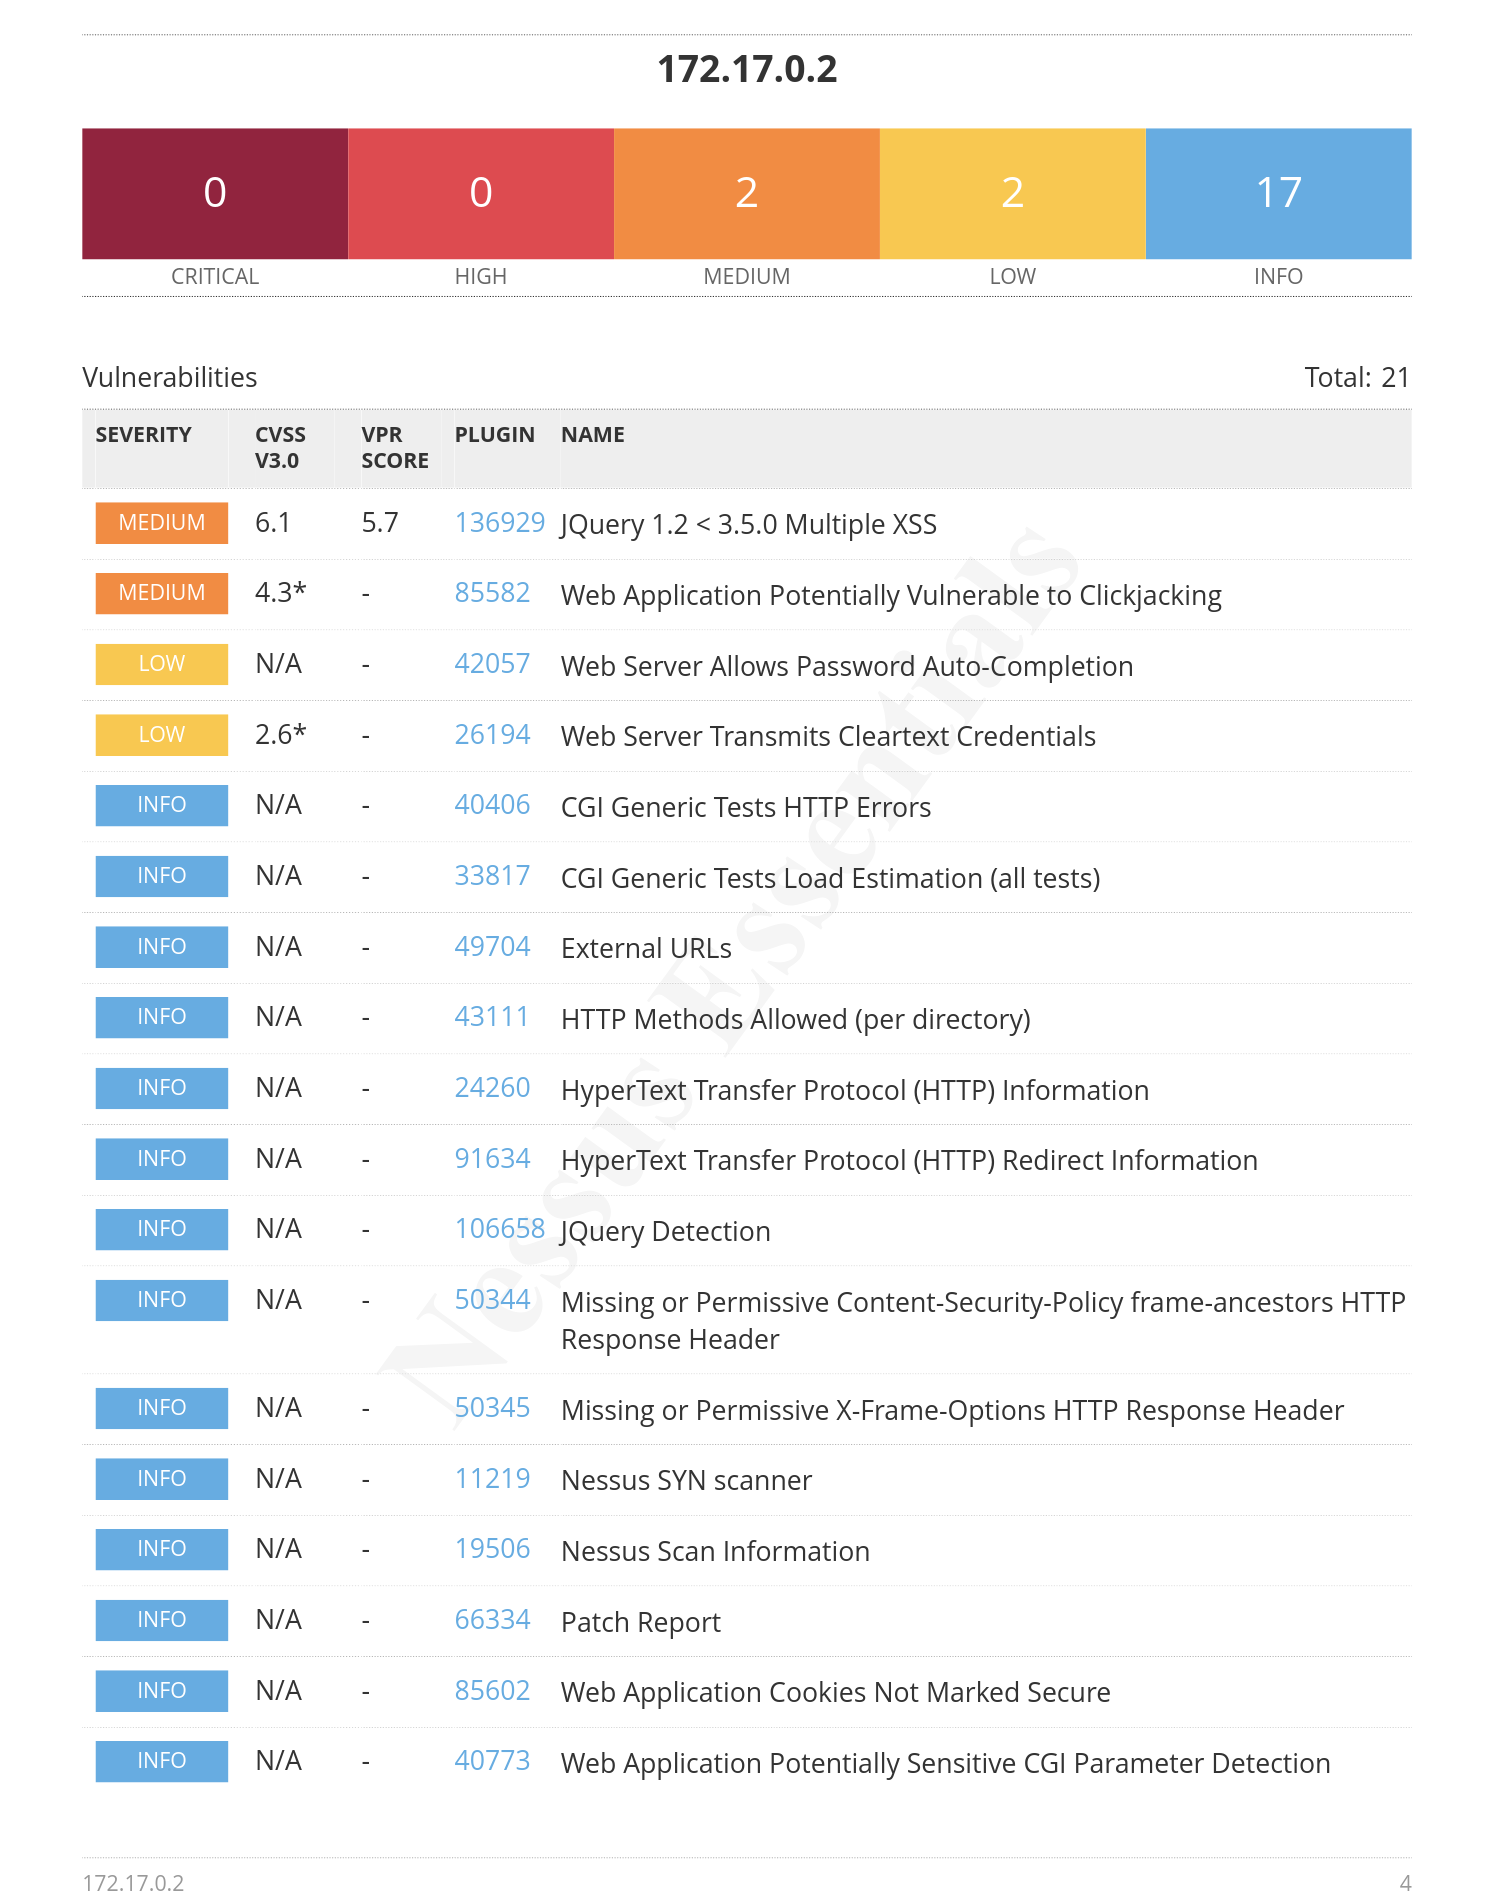
\includegraphics[width=\linewidth]{img/nessus-dvna-before.png}
%   \caption{Wyniki skanowania aplikacji DVNA przy użyciu skanera Nessus}
%   \label{fig:nessus-dvna-before}
% \end{figure}
% \begin{figure}[H]
%   \centering
%   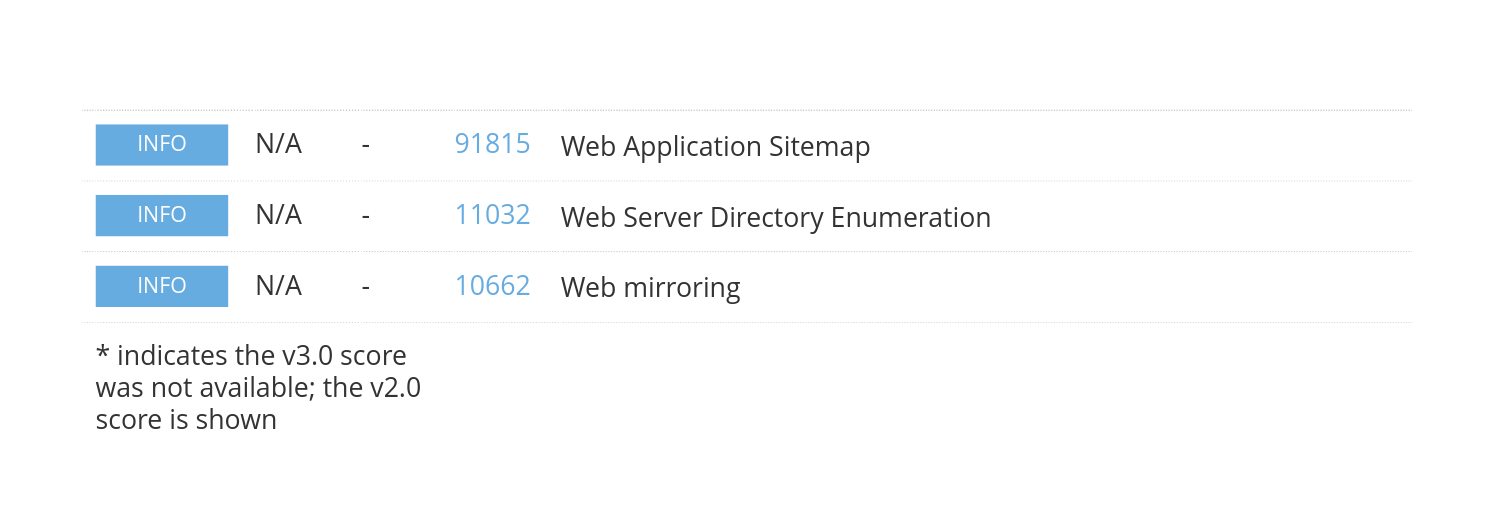
\includegraphics[width=\linewidth]{img/nessus-dvna-before2.png}
%   \caption{Wyniki skanowania aplikacji DVNA przy użyciu skanera Nessus}
%   \label{fig:nessus-dvna-before2}
% \end{figure}

% \section{Analiza statyczna i naprawa}

% Z wykorzystaniem narzędzia \texttt{gptester} przeprowadzono szczegółową analizę statyczną kodu źródłowego DVNA. Proces ten skupiał się na identyfikacji znanych podatności z listy OWASP Top 10 oraz sugerowaniu możliwych napraw. Po zakończeniu analizy, \texttt{gptester} wygenerował zestaw rekomendacji, które zostały zaimplementowane w kodzie źródłowym aplikacji w celu usunięcia zidentyfikowanych słabości.

% \begin{verbatim}
%   Found 77 files to scan
%   Tokens inside the directory: 22694
% \end{verbatim}

% \texttt{GPTester} znalazł 77 plików do przeskanowania, zawierających łącznie 22694 tokenów. 

% \section{Weryfikacja i ocena skuteczności}

% Po wprowadzeniu sugerowanych zmian, aplikacja DVNA została ponownie poddana skanowaniu przy użyciu skanerów OWASP ZAP i Nessus, aby ocenić skuteczność wprowadzonych modyfikacji. Wyniki tego ponownego skanowania zostały porównane z wynikami początkowymi, co pozwoliło na ocenę efektywności narzędzia \texttt{gptester} w kontekście naprawy podatności.

% \section{Wyniki i dyskusja}

% Analiza wyników wskazała na zauważalną poprawę bezpieczeństwa aplikacji DVNA po zastosowaniu napraw sugerowanych przez \texttt{gptester}. W większości przypadków narzędzie skutecznie zidentyfikowało podatności i zaproponowało adekwatne rozwiązania, które pozytywnie przyczyniły się do zmniejszenia ogólnego ryzyka bezpieczeństwa aplikacji.

% \subsection{Wyzwania i ograniczenia}

% Jednakże, nie wszystkie sugerowane zmiany były w pełni skuteczne lub odpowiednie dla specyfiki aplikacji DVNA. W niektórych przypadkach, wprowadzenie zmian wymagało dodatkowej analizy i dostosowania sugerowanych rozwiązań do kontekstu aplikacji. Ponadto, niektóre z bardziej złożonych podatności wymagały bardziej zaawansowanych metod naprawczych, co wykraczało poza możliwości automatycznej analizy statycznej.

% \section{Wnioski}

% Badanie potwierdziło potencjał wykorzystania narzędzia \texttt{gptester} wspieranego przez zaawansowane modele językowe w procesie identyfikacji i naprawy podatności w aplikacjach webowych. Mimo pewnych ograniczeń, narzędzie to stanowi wartościowe wsparcie w procesie zapewniania bezpieczeństwa aplikacji, szczególnie w kontekście szybkiego wykrywania i łagodzenia powszechnych podatności. Dalszy rozwój narzędzia, w tym lepsza integracja z kontekstem aplikacji i zaawansowane metody naprawcze, może znacznie zwiększyć jego skuteczność i przydatność w praktycznych zastosowaniach.

% \chapter{Badanie funkcjonalności na aplikacji webowej OWASP VulnerableApp}
% \label{sec:badania_na_aplikacji_webowej_owasp}

% Analiza funkcjonalności programu do analizy bezpieczeństwa została przeprowadzona z wykorzystaniem aplikacji webowej OWASP VulnerableApp. Jest to narzędzie celowo zawierające liczne podatności, które mają na celu symulację realnych luk bezpieczeństwa, co pozwala na dogłębne testowanie i ocenę narzędzi do skanowania podatności.

% \section{Charakterystyka aplikacji OWASP VulnerableApp}
% Aplikacja OWASP VulnerableApp została zaprojektowana z myślą o dostarczeniu platformy edukacyjnej dla deweloperów oraz specjalistów od bezpieczeństwa, którzy pragną zgłębić wiedzę na temat bezpieczeństwa aplikacji webowych. Narzędzie to charakteryzuje się skalowalnością, elastycznością oraz łatwością integracji, czyniąc je idealnym środowiskiem do nauki oraz testowania.

% \section{Testowane rodzaje podatności}
% OWASP VulnerableApp umożliwia testowanie szerokiego zakresu podatności, w tym, ale nie ograniczając się do:
% \relax
% \begin{itemize}
%     \item Podatności JWT
%     \item Wstrzykiwanie poleceń (Command Injection)
%     \item Podatności związane z przesyłaniem plików (File Upload Vulnerability)
%     \item Przejście ścieżki (Path Traversal)
%     \item Iniekcje SQL (SQL Injection)
%     \item Skrypty międzywitrynowe (XSS)
%     \item Ataki oparte na External XML Entities (XXE)
%     \item Open Redirect
%     \item Server-Side Request Forgery (SSRF)
% \end{itemize}

% Zawarte podatności są reprezentatywne dla typowych zagrożeń w aplikacjach internetowych, co pozwala na wszechstronne i realistyczne testowanie narzędzi do ich wykrywania i naprawy.

% \section{Zawartość znajdująca się w repozytorium}
% Repozytorium aplikacji VulnerableApp zawiera projekt aplikacji webowej napisany w następującym stosie technologicznym:
% \begin{itemize}
%     \item Java 8
%     \item Spring Boot
%     \item Maven 3.6.1
%     \item ReactJS
%     \item Javascript/TypeScript
% \end{itemize} 

% \begin{verbatim}
%  > ./main.py ../testing-envs/VulnerableApp/

%                   ___  ___  _____           _             
%                  / __|| _ \|_   _| ___  ___| |_  ___  _ _ 
%                 | (_ ||  _/  | |  / -_)(_-/|  _|/ -_)| '_|
%                  \___||_|    |_|  \___|/__/ \__|\___||_|  

%            The static code analysis agent, version: assistant-0.3


% 2024-01-25 22:05:23: Beginning scan for ../testing-envs/VulnerableApp/
% 2024-01-25 22:05:23: Found 97 files to scan
% 2024-01-25 22:05:23: Tokens inside the directory: 77513
% 2024-01-25 22:05:23: Using model: gpt-4-1106-preview
% 2024-01-25 22:05:23: Beginning code analysis...
% \end{verbatim}

% W repozytorium znajduje się 231 plików, które zawierają 229119 tokenów z uwzględnieniem wszystkich plików. Nasz program pokazał wartości dla plików zawierających kod, a dokładnie tych które nie są wyspecjalizowane w liście nazw do ignorowania.

% \section{Procedura przeprowadzenia testów}
% Testy zostały przeprowadzone przy użyciu najnowszej wersji programu, zgodnie z następującymi krokami:

% \begin{enumerate}
%     \item Przygotowanie środowiska testowego z wykorzystaniem aplikacji OWASP VulnerableApp.
%     \item Uruchomienie skanowania z wykorzystaniem programu.
%     \item Dokumentacja wykrytych podatności oraz sugerowanych przez program napraw.
%     \item Analiza efektywności napraw i ich wpływ na bezpieczeństwo aplikacji za pomocą innych skanerów podatności.
% \end{enumerate}

% \subsection{Oczekiwane rezultaty}
% W wyniku przeprowadzonych testów oczekujemy uzyskania szczegółowych danych na temat liczby wykrytych podatności, rodzajów podatności, a także czasu potrzebnego na ich wykrycie i naprawę. Dane te zostaną następnie wykorzystane do stworzenia szczegółowych wykresów i tabel ilustrujących skuteczność programu.

% \section{Wnioski i dalsze kierunki badań}
% Na podstawie zebranych danych zostaną wyciągnięte wnioski dotyczące skuteczności narzędzia w kontekście poszczególnych typów podatności oraz ogólnej wydajności. Dalsze badania mogą również koncentrować się na porównaniu wyników z innymi narzędziami dostępnymi na rynku oraz na rozwoju nowych funkcji i usprawnień w badanym programie.

\chapter{Przeprowadzenie testów na aplikacji NodeGoat}

\section{Wstęp}
\label{sec:wstep}
W ramach niniejszego rozdziału zostanie przeanalizowana aplikacja NodeGoat, służąca do edukacji w zakresie zabezpieczeń aplikacji internetowych opartych na platformie Node.js. NodeGoat, będąc projektowaną z myślą o nauce i praktyce, oferuje środowisko, w którym użytkownicy mogą eksplorować i naprawiać najczęściej występujące luki bezpieczeństwa określone w ramach OWASP Top 10 dla aplikacji webowych.

Node.js, jako lekka, szybka i skalowalna platforma, która zyskuje coraz większą popularność wśród deweloperów aplikacji internetowych. Z tego względu narzędzia takie jak NodeGoat odgrywają kluczową rolę w edukacji z zakresu bezpieczeństwa, umożliwiając użytkownikom praktyczne zrozumienie zagrożeń i metod ich przeciwdziałania.
\\

\textbf{Przeznaczenie aplikacji}

NodeGoat zapewnia kompleksowy tutorial, który opisuje poszczególne zagrożenia z listy OWASP Top 10, demonstrując je na przykładzie działającej aplikacji. Użytkownicy mają możliwość nie tylko zapoznania się z teorią, ale również praktycznego przetestowania każdego z zagrożeń, co stanowi cenny element edukacyjny.
\\

\textbf{Praktyczne testowanie zabezpieczeń}

Aplikacja NodeGoat została zaprojektowana z celowymi słabościami bezpieczeństwa, dzięki czemu użytkownicy mogą w bezpiecznym środowisku przeprowadzać ataki i testować różne techniki obronne. Dostęp do aplikacji jest możliwy lokalnie, co umożliwia dogłębne badanie kodu oraz modyfikowanie go w celu naprawy istniejących luk. Zaimplemntowano również zaawansowany moduł testów funkcjonalnych, który pozwala na automatyczne przeprowadzanie testów funkcjonalności i ocenę poprawności zastosowanych metod naprawczych.
\\

\textbf{Konta użytkowników}

Domyślnie, baza danych aplikacji zawiera predefiniowane konta użytkowników, w tym konto administratora oraz kilka kont użytkowników zwykłych. Umożliwia to szybkie rozpoczęcie testowania aplikacji bez konieczności ręcznego konfigurowania środowiska.\\

W niniejszym rozdziale szczegółowo przedstawione zostaną metody testowania aplikacji NodeGoat, wykorzystując do analizy duże modele językowe. Przeprowadzone badania mają na celu nie tylko identyfikację istniejących słabości, ale również ocenę skuteczności zastosowanych metod naprawczych.

\section{Przygotowanie środowiska testowego}
\label{sec:przygotowanie_srodowiska_testowego}

Aby przygotować aplikację do lokalnego uruchomienia bez korzystania z konteneryzacji, niezbędne było poprawienie wersji paczek w pliku package.json oraz obniżenie używanej wersji npm i node do node v16.0.0 (npm v7.10.0). Następnie należało zainstalować wszystkie zależności za pomocą komendy npm install. Po wykonaniu tych kroków aplikacja była gotowa do uruchomienia komendą \texttt{npm start}.

\section{Testy funkcjonalne przed zmianami}
\label{sec:testy_funkcjonalne_przed_zmianami}

\begin{figure}[H]
  \centering
  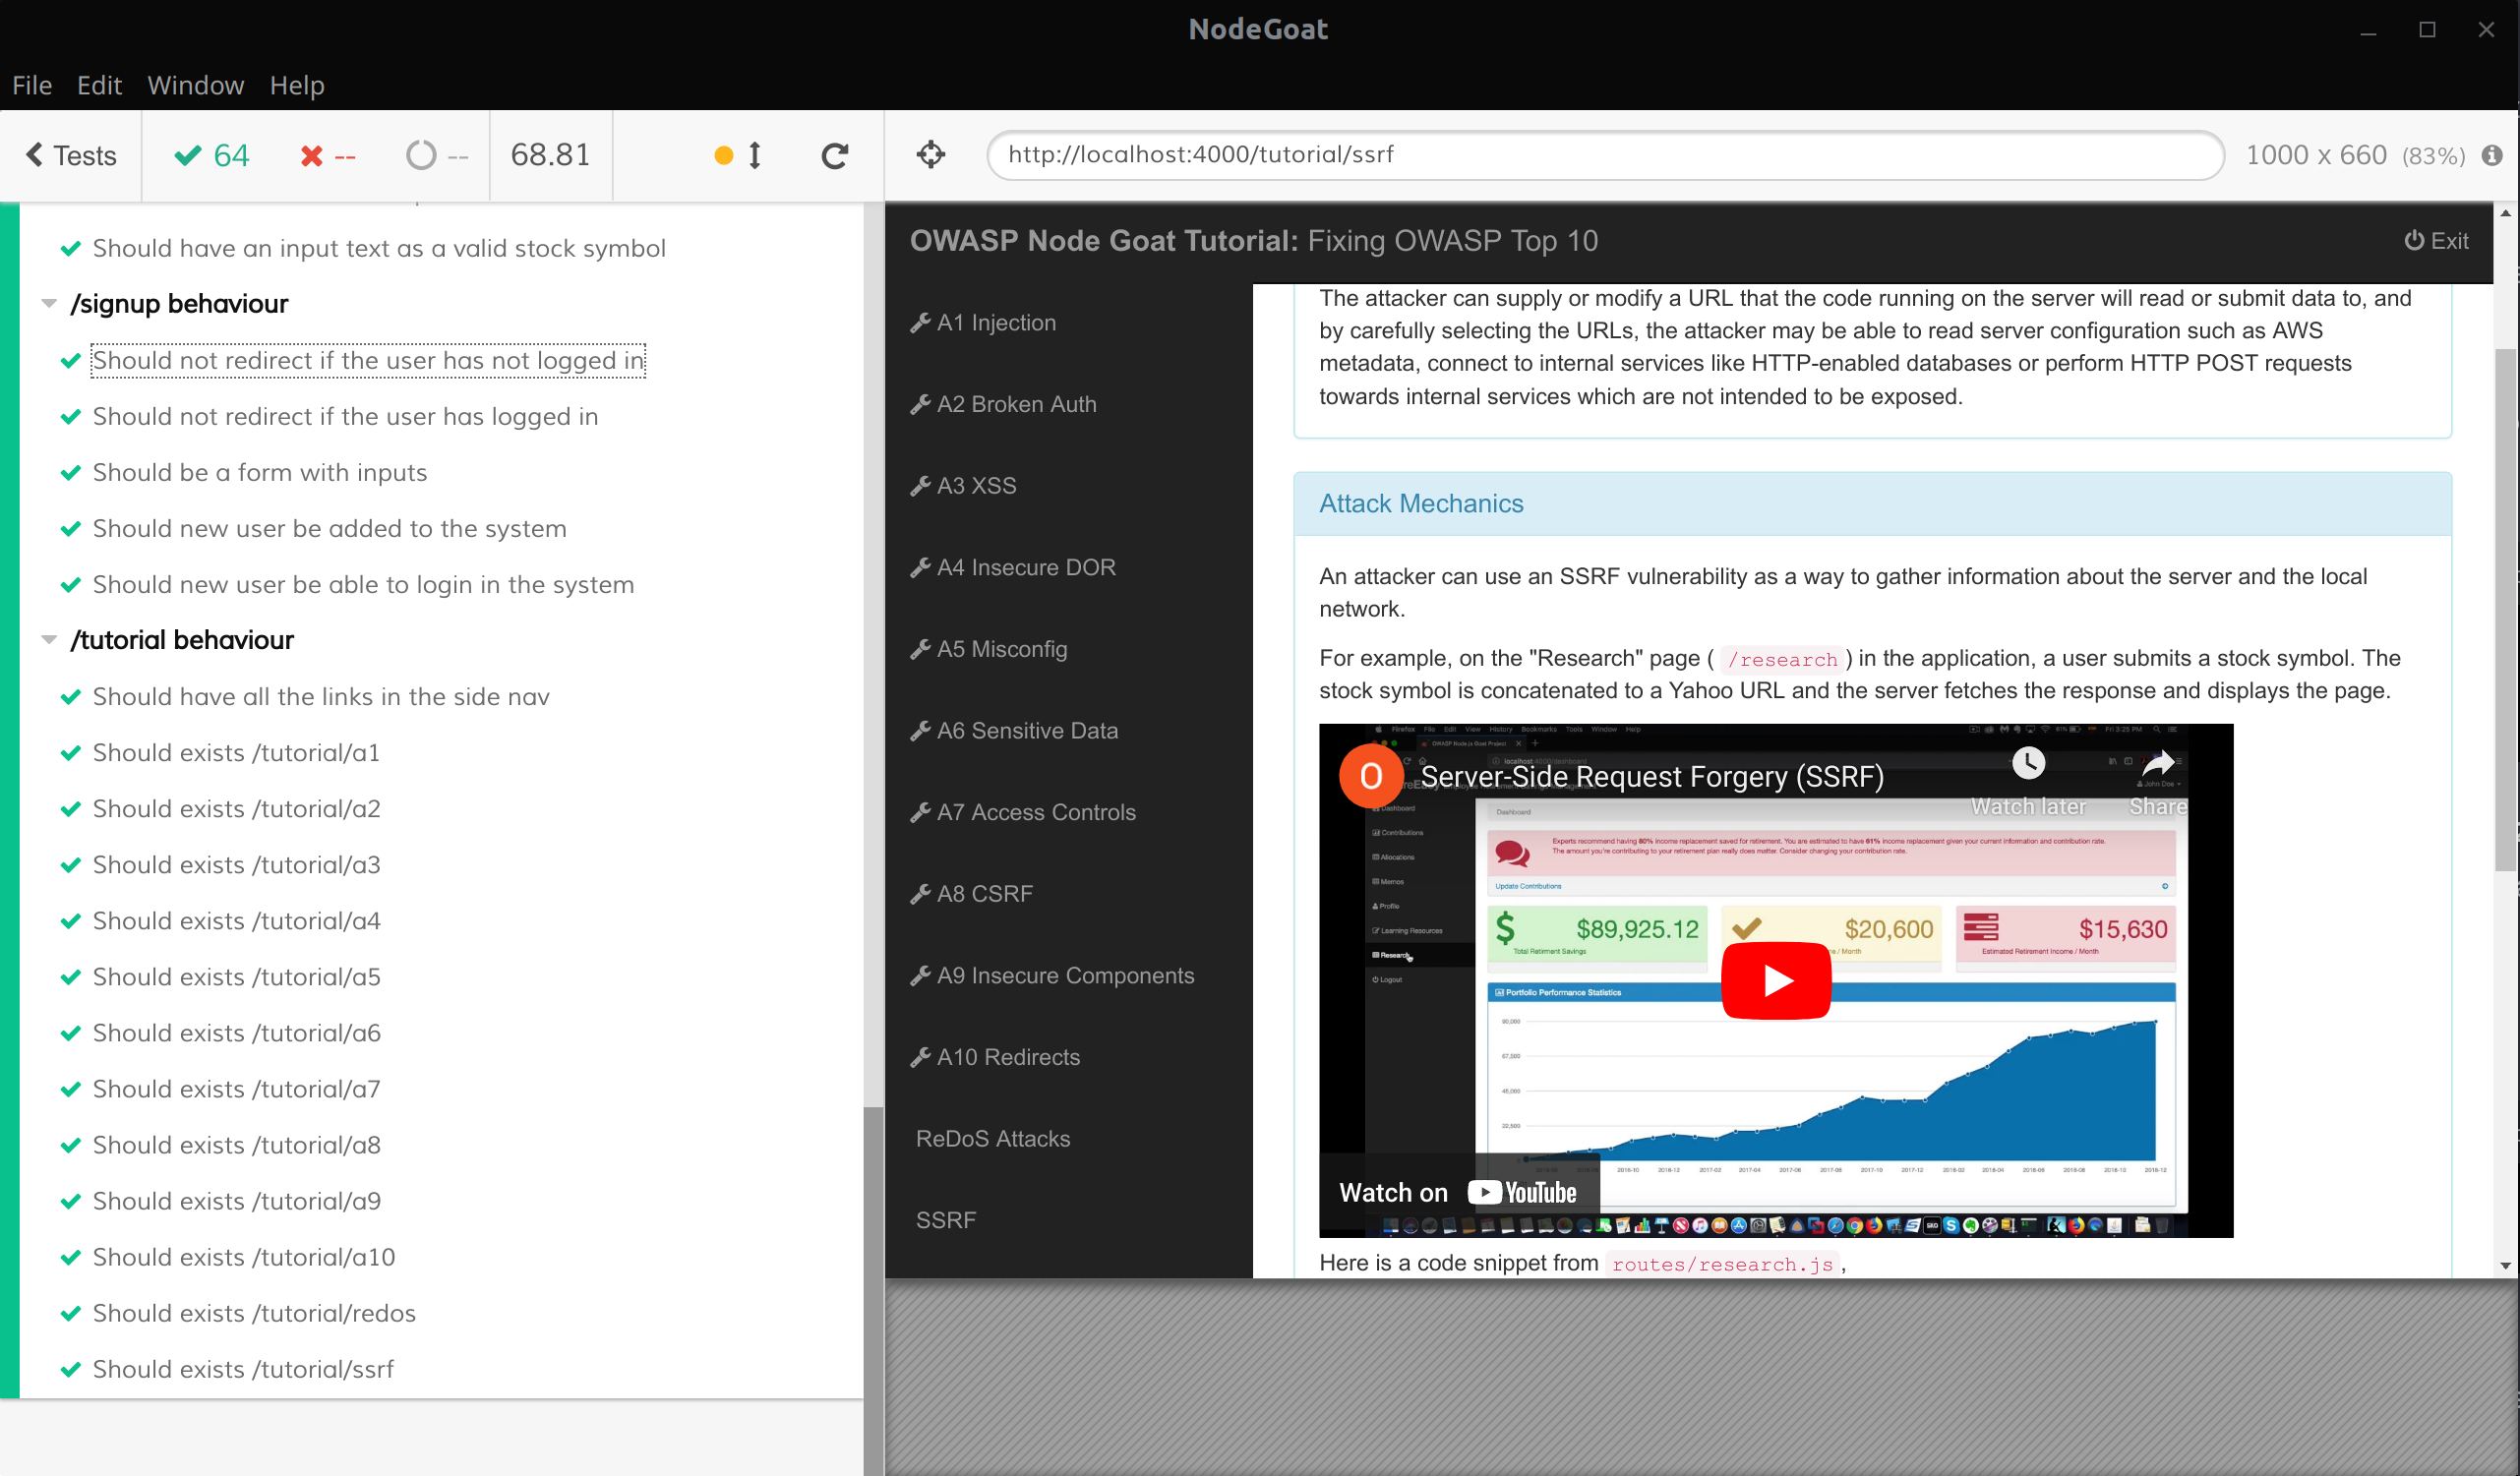
\includegraphics[width=\linewidth]{img/func-test-goat-before.png}
  \caption{Wyniki testów funkcjonalnych aplikacji NodeGoat przed wprowadzeniem zmian}
  \label{fig:nodegoat-before}
\end{figure}

\section{Identyfikacja podatności za pomocą tradycyjnych skanerów}
Przed przystąpieniem do naprawy podatności, aplikacja DVNA została poddana skanowaniu przy użyciu skanerów OWASP ZAP i Nessus. Wyniki tych skanowań zostały wykorzystane jako punkt odniesienia do oceny skuteczności narzędzia \texttt{gptester} w kontekście naprawy podatności.


\subsection{OWASP ZAP}
\label{subsec:owasp_zap}
Skanowanie aplikacji NodeGoat przy użyciu OWASP ZAP wykazało obecność 20 podatności, w tym 3 krytyczne, 5 wysokiego ryzyka, 5 średniego ryzyka oraz 7 niskiego ryzyka. Poniżej przedstawiono listę zidentyfikowanych podatności wraz z ich ryzykiem i opisem.

\begin{table}[H]
  \caption{Wyniki skanowania aplikacji NodeGoat przy użyciu skanera \texttt{OWASP-zap}}
  \begin{tabular}{llllll}
    \multicolumn{2}{l}{} &
      \multicolumn{4}{c}{Risk} \\ \cline{3-6} 
    \multicolumn{2}{l|}{} &
      \multicolumn{1}{l|}{\begin{tabular}[c]{@{}l@{}}High\\ (= High)\end{tabular}} &
      \multicolumn{1}{l|}{\begin{tabular}[c]{@{}l@{}}Medium\\ (\textgreater{}= Medium)\end{tabular}} &
      \multicolumn{1}{l|}{\begin{tabular}[c]{@{}l@{}}Low\\ (\textgreater{}= Low)\end{tabular}} &
      \multicolumn{1}{l|}{\begin{tabular}[c]{@{}l@{}}Informational\\ (\textgreater{}= Informational)\end{tabular}} \\ \cline{2-6} 
    \multicolumn{1}{l|}{site} &
      \multicolumn{1}{l|}{http://localhost:4000} &
      \multicolumn{1}{l|}{\begin{tabular}[c]{@{}l@{}}3\\ (3)\end{tabular}} &
      \multicolumn{1}{l|}{\begin{tabular}[c]{@{}l@{}}5\\ (8)\end{tabular}} &
      \multicolumn{1}{l|}{\begin{tabular}[c]{@{}l@{}}5\\ (13)\end{tabular}} &
      \multicolumn{1}{l|}{\begin{tabular}[c]{@{}l@{}}7\\ (20)\end{tabular}} \\ \cline{2-6} 
    \end{tabular}   
  \label{tab:zap_before}
  \end{table}

  \begin{table}[htbp]
    \centering
    \scriptsize
    \caption{Podsumowanie typów alertów i powiązanych zagrożeń}
    \label{tab:alert_summary}
    \begin{tabular}{|l|l|r|}
    \hline
    \textbf{Alert Type} & \textbf{Risk} & \textbf{Count (\%)} \\
    \hline
    Cross Site Scripting (Reflected) & High & 3 (15.0\%) \\
    External Redirect & High & 1 (5.0\%) \\
    Open Redirect & High & 1 (5.0\%) \\
    CSP: Wildcard Directive & Medium & 16 (80.0\%) \\
    Content Security Policy (CSP) Header Not Set & Medium & 24 (120.0\%) \\
    Directory Browsing & Medium & 2 (10.0\%) \\
    Missing Anti-clickjacking Header & Medium & 24 (120.0\%) \\
    Vulnerable JS Library & Medium & 2 (10.0\%) \\
    Cookie without SameSite Attribute & Low & 5 (25.0\%) \\
    Cross-Domain JavaScript Source File Inclusion & Low & 24 (120.0\%) \\
    Server Leaks Information via "X-Powered-By" HTTP Response Header Field(s) & Low & 63 (315.0\%) \\
    Timestamp Disclosure - Unix & Low & 1 (5.0\%) \\
    X-Content-Type-Options Header Missing & Low & 37 (185.0\%) \\
    Authentication Request Identified & Informational & 1 (5.0\%) \\
    Information Disclosure - Suspicious Comments & Informational & 26 (130.0\%) \\
    Loosely Scoped Cookie & Informational & 5 (25.0\%) \\
    Modern Web Application & Informational & 23 (115.0\%) \\
    Session Management Response Identified & Informational & 8 (40.0\%) \\
    User Agent Fuzzer & Informational & 290 (1,450.0\%) \\
    User Controllable HTML Element Attribute (Potential XSS) & Informational & 2 (10.0\%) \\
    \hline
    \textbf{Total} & & \textbf{Various} \\
    \hline
    \end{tabular}
    \end{table}
    
\normalsize
\subsection{Statyczny analizator CodeQL}\label{subsec:codeql}

\subsubsection{Proces przeprowadzenia testu}

\begin{enumerate}
    \item Przygotowanie środowiska testowego dla aplikacji NodeGoat.
    
    

    \item Uruchomienie skanowania z wykorzystaniem programu.
    Przed przystąpieniem do skanowania należy utworzyć bazę danych CodeQL. W tym celu należy wykonać następujące kroki:
    \begin{enumerate}
        \item Zainstalować CodeQL CLI.
        \item Zainicjalizować i zbudować bazę danych CodeQL. \\\\
        \scriptsize
        \begin{adjustwidth}
        {-2cm}{}
        \begin{verbatim}
> codeql database create GoatQL-db --language=javascript  
Initializing database at /home/paris/projekty/INZYNIERKA/testing-envs/NodeGoat/GoatQL-db.
Running build command: []
[2024-01-25 19:33:30] [build-stdout] Single-threaded extraction.
[2024-01-25 19:33:34] [build-stdout] package.json: Main file set to server.js
[2024-01-25 19:33:34] [build-stdout] Extracting .../NodeGoat/app/views/tutorial/a1.html
[2024-01-25 19:33:34] [build-stdout] Done extracting .../NodeGoat/app/views/tutorial/a1.html (91 ms)
[2024-01-25 19:33:34] [build-stdout] Extracting .../NodeGoat/app/views/tutorial/a10.html
[2024-01-25 19:33:34] [build-stdout] Done extracting .../NodeGoat/app/views/tutorial/a10.html (5 ms)
[2024-01-25 19:33:34] [build-stdout] Extracting .../NodeGoat/app/views/tutorial/a2.html
.
.
.
[2024-01-25 19:33:38] [build-stdout] Extracting .../codeql/javascript/tools/data/externs/nodejs/vm.js
[2024-01-25 19:33:38] [build-stdout] Done extracting .../codeql/javascript/tools/data/externs/nodejs/vm.js (8 ms)
Finalizing database at /home/paris/projekty/INZYNIERKA/testing-envs/NodeGoat/GoatQL-db.
Successfully created database at /home/paris/projekty/INZYNIERKA/testing-envs/NodeGoat/GoatQL-db.
        \end{verbatim}
      \end{adjustwidth}
        \normalsize
        \item Uruchomić wybrane zapytania na bazie danych wyszukujące podatności.
        
        W tym celu uruchomiłem domyślne pakiety zapytań dostępne w CodeQL CLI. W celu uruchomienia zapytania należy wykonać następującą komendę: \\\\
        \scriptsize
        \begin{adjustwidth}
        {-2cm}{}
        \begin{verbatim}
> codeql database analyze GoatQL-db javascript-code-scanning.qls --format=csv --output=default-goat-QLresults.csv
Running queries.
[1/88] Loaded .../codeql/javascript-queries/0.8.2/AngularJS/InsecureUrlWhitelist.qlx.
        \end{verbatim}
      \end{adjustwidth}
      \normalsize
        Komenda zakończyła się sukcesem, a w katalogu pojawił się plik z wynikami analizy. \\\\
        \scriptsize
        \begin{adjustwidth}
        {-2cm}{}
        \begin{verbatim}
PrototypePollutingFunction.ql            : [83/88 eval 25ms] Results written to codeql/javascript-queri
PrototypePollutingMergeCall.ql           : [84/88 eval 260ms] Results written to codeql/javascript-quer
InsufficientPasswordHash.ql              : [85/88 eval 5ms] Results written to codeql/javascript-querie
RequestForgery.ql                        : [86/88 eval 143ms] Results written to codeql/javascript-quer
LinesOfCode.ql                           : [87/88 eval 3ms] Results written to codeql/javascript-querie
LinesOfUserCode.ql                       : [88/88 eval 644ms] Results written to codeql/javascript-quer
Shutting down query evaluator.
Interpreting results.
Analysis produced the following diagnostic data:

|          Diagnostic          |  Summary   |
+------------------------------+------------+
| Successfully extracted files | 77 results |

Analysis produced the following metric data:

|                                   Metric                                   | Value |
+----------------------------------------------------------------------------+-------+
| Total lines of user written JavaScript and TypeScript code in the database |  2926 |
| Total lines of JavaScript and TypeScript code in the database              |  2932 |
\end{verbatim}
\end{adjustwidth}
\normalsize\\
\vspace*{1cm}
Na aplikacji został również uruchomiony pakiet kwerend javascript-extended-security.qls \\
    \end{enumerate}

    \item Dokumentacja wykrytych podatności oraz sugerowanych przez program napraw.
    \item Analiza efektywności napraw i ich wpływ na bezpieczeństwo aplikacji za pomocą innych skanerów podatności.
\end{enumerate}

\subsection{Wyniki otrzymane z analizy CodeQL}
\begin{table}[H]
  \centering
  \caption{Podsumowanie wyników analizy CodeQL}
  \label{table:regex_vulnerabilities}
  \resizebox{\textwidth}{!}{%
  \begin{tabular}{|l|l|l|l|}
    \hline
    \textbf{Issue} & \textbf{Description} & \textbf{File} & \textbf{Occurrences} \\ \hline
    Inefficient regular expression & Can cause exponential backtracking & profile.js & 1 \\ \hline
    Polynomial regex on uncontrolled data & May be vulnerable to DoS attacks & profile.js, session.js & 2 \\ \hline
    Database query from user input & Risk of malicious code insertion & user-dao.js & 2 \\ \hline
    Clear text sensitive cookie transmission & Sensitive cookies sent without SSL & server.js & 1 \\ \hline
    Missing CSRF middleware & Lack of CSRF protection risks malicious requests & server.js & Multiple \\ \hline
    Server-side URL redirect & May redirect to malicious websites & index.js & 1 \\ \hline
    Code injection & Allows arbitrary code execution by a user & contributions.js & Multiple \\ \hline
    Missing rate limiting & Vulnerable to DoS attacks & index.js & 1 \\ \hline
    Server-side request forgery & User-controlled data in URL risks forgery attacks & research.js & 1 \\ \hline
    DOM text as HTML & Leads to XSS vulnerability & bootstrap.js & Multiple \\ \hline
    Unsafe jQuery plugin & Constructs HTML unsafely, risking XSS & bootstrap.js & Multiple \\
    \hline
  \end{tabular}}
\end{table}
Rozszerzony pakiet kwerend rozszerzył wyniki o następujące wpisy:

\begin{table}[!ht]
  \centering
  \caption{Extended Scanning Results with CodeQL}
  \label{table:codeql_extended_results}
  \resizebox{\textwidth}{!}{%
  \begin{tabular}{|l|l|l|l|}
    \hline
    \textbf{Issue} & \textbf{Description} & \textbf{File} & \textbf{Details} \\ \hline
    Failure to abandon session & Reuse of session can lead to account access & index.js & Session not invalidated post-login \\ \hline
    Log injection & Forged log entries risk from user inputs & session.js & Log entry built from user input \\ \hline
    Indirect command line in shell & May introduce command-line injection vulnerabilities & Gruntfile.js & Command depends on unsanitized env variable \\
    \hline
  \end{tabular}}
\end{table}


\section{Analiza GPTester z wykorzystaniem RAG}
Z uwagi na wielkość projektu i limit dla API asystentów wynoszący 32768 znaków (nie tokenów), kod był przetwarzany przez aplikację w aż 50 częściach asynchronicznie. Wykorzystana została dodatkowo funkcja generacji wspomaganej pobieraniem danych. 

Niestety firmowy klucz API OpenAI, z którego korzystałem by wykonać skan został pod sam koniec wycofany, prawdopobnie przez dużą liczbę zapytań. W związku z tym, udało się przeprowadzić skanowanie tylko dla ~45 części kodu, co stanowiło około 9/10 kodu aplikacji. Skanowanych było o 10 plików więcej niż uwzględniał CodeQL, co wynikało z faktu, że CodeQL nie uwzględniał plików konfiguracyjnych i tych które zawierały kod HTML. 
Pozwoliło to agentowi na aktualizację wersji oprogramowania w plikach konfiguracyjnych.

Ze względu na zwiększone koszta związane z wysyłaniem tylu zapytań do OpenAI i ograniczenia czasowe zoptymalizowałem kod tak, aby skanowanie odbywało się ignorując pliki nie zawierające kodu. Tę konfigurację można edytować z pomocą pliku \texttt{config.py}.
\section{Analiza GPTester bez RAG}
Następnie uruchomiłem proces analizy kodu za pomocą GPTester bez użycia RAG. W tym celu wykorzystałem prywatny klucz API OpenAI, dzięki czemu mogłem dowiedzieć się jakie koszty są generowane podczas skanowania. Zoptymalizowałem także wybieranie plików do skanowania, aby ograniczyć koszty. 
W sumie GPTester znalazł 21 podatności, bez określania ich ryzyka. Wśród nich były podatności takie jak:\\


\begin{enumerate}
  \item[1.] \textbf{Hardcoded Sensitive Information}: The \texttt{db-reset.js} file contains hardcoded sensitive information such as usernames and passwords that should not be stored in plain text. This is a security risk as it can be exploited if the code is exposed.
  \item[2.] \textbf{Insecure Randomness}: The \texttt{db-reset.js} file generates random allocation percentages using \texttt{Math.random()}, which is not cryptographically secure and thus not suitable for security-sensitive contexts.
  \item[3.] \textbf{Unvalidated Redirects and Forwards}: The \texttt{index.js} file uses query parameter \texttt{url} to redirect the user without validation in the \texttt{/learn} route. This can lead to phishing attacks or redirection to malicious sites.
  \item[4.] \textbf{Insecure Direct Object References (IDOR)}: The \texttt{allocations.js} file uses \texttt{req.params.userId} directly from the URL, which allows users to access other users' allocation data without proper authorization.
  \item[5.] \textbf{Server-Side JavaScript Injection (SSJI)}: The \texttt{contributions.js} file uses an insecure \texttt{eval()} function to parse user inputs, which could allow an attacker to run arbitrary code on the server.
  \item[6.] \textbf{Cross-Site Scripting (XSS)}: The \texttt{profile.js} file attempts to encode user-supplied input with \texttt{ESAPI.encoder().encodeForHTML(doc.website)} which could lead to XSS attacks if not properly encoded for the context in which it is rendered.
  \item[7.] \textbf{Regular Expression Denial of Service (ReDoS)}: The \texttt{profile.js} file uses a vulnerable regular expression that may cause the application to freeze with specially crafted input. \\
  \item[1.] Log Injection Vulnerability - In the \texttt{handleLoginRequest} method in \texttt{session.js}, user input (\texttt{userName}) is being logged without proper sanitization, which can be exploited by an attacker to forge logs or execute code.
  \item[2.] Insecure Password Storage - In \texttt{user-dao.js}, the \texttt{addUser} method stores passwords as plain text, which is insecure as it can be easily read if the database is compromised.
  \item[3.] Session Fixation - In \texttt{session.js}, the method \texttt{handleLoginRequest} doesn't regenerate the session ID after a successful login, making the application vulnerable to session fixation attacks.
  \item[4.] NoSQL Injection - The method \texttt{getByUserIdAndThreshold} in \texttt{allocations-dao.js} constructs a query using string concatenation without properly sanitizing the \texttt{threshold} parameter, making it susceptible to NoSQL injection attacks.
  \item[5.] Insufficient Password Strength Validation - The \texttt{validateSignup} method in \texttt{session.js} uses a regular expression for password validation, but the commented out regex suggests that a stronger password policy was considered and not implemented.
  \item[6.] Sensitive Data Exposure - In \texttt{profile-dao.js}, sensitive information like \texttt{ssn} and \texttt{dob} are stored without encryption, which makes them vulnerable to exposure if there is a data breach. \\
  \item[1.] Insecure Database Connection (\texttt{../testing-envs/NodeGoat/server.js}) - The \texttt{MongoClient.connect} call uses a connection string that might not be secure. The code for setting up the database connection does not include SSL/TLS configuration options which are important for secure transmission of data over the network.
  \item[2.] Server-Side Template Injection (\texttt{../testing-envs/NodeGoat/server.js}) - The template engine Swig is used without autoescaping enabled, this could lead to Server-Side Template Injection (SSTI) if the template rendering includes user input.
  \item[3.] HTTP Connection (\texttt{../testing-envs/NodeGoat/server.js}) - The server is started with an insecure HTTP connection instead of HTTPS, which exposes the transmitted data to potential interception and tampering.
  \item[4.] Insufficient Session Management (\texttt{../testing-envs/NodeGoat/server.js}) - The session is created with \texttt{saveUninitialized: true}, which can lead to the generation of session identifiers even when the session is not actually started for the user.
  \item[5.] Lack of Cookie Security (\texttt{../testing-envs/NodeGoat/server.js}) - No secure flags for cookies are set like \texttt{httpOnly} and \texttt{secure}. This can make the session cookies vulnerable to XSS attacks and interception over insecure connections.
  \item[6.] Lack of Security Headers (\texttt{../testing-envs/NodeGoat/server.js}) - Security headers such as Content Security Policy (CSP), X-Frame-Options, X-XSS-Protection, and others are commented out. This could lead to various attacks such as clickjacking, XSS, etc.
  \item[7.] Insecure Static File Permissions (\texttt{../testing-envs/NodeGoat/docker-compose.yml}) - The Dockerfile setup for the NodeGoat container runs commands as the root user, which can be a security risk if the container is compromised.
  \item[8.] Incomplete Logging Configuration (\texttt{../testing-envs/NodeGoat/Gruntfile.js}) - The Grunt configuration does not include tasks for security logging or monitoring, which can leave the application without proper tracking of security-related events.
\end{enumerate}
Wyniki zostały przedstawione w częściach, tak jak były przetwarzane, bez modyfikacji ani tłumaczenia. Dla klarowności przedstawionych wyników została dodana funkcjonalność zapisu do pliku csv.

\section{Wprowadzanie zmian w kodzie}
Po przeprowadzeniu analiz kodu, należało wprowadzić zmiany w kodzie, które miały naprawić wykryte podatności. W tej wersji program dostarczył 38 nowych plików. W nowych wersjach ilość analizowanych plików została zoptymalizowana ze względu na koszty.
\subsection{Wprowadzenie zmian za pomocą skryptu}
Z uwagi na ciągłe dopracowywanie funkcji aktualizacji kodu za pomocą funkcji git, napisano prosty skrypt bash (\texttt{gptester/utils/replace\_files.sh}), który zamieniał pliki o tych samych nazwach. Niestety plików z tymi samymi nazwami jest kilka w oryginalnym projekcie co doprowadziło do wielokrotnej zamiany i błędów uruchomienia aplikacji. Wiele z otrzymanych plików miało jedynie część kodu, co uniemożliwiło uruchomienie aplikacji.

\begin{figure}[H]
  \centering
  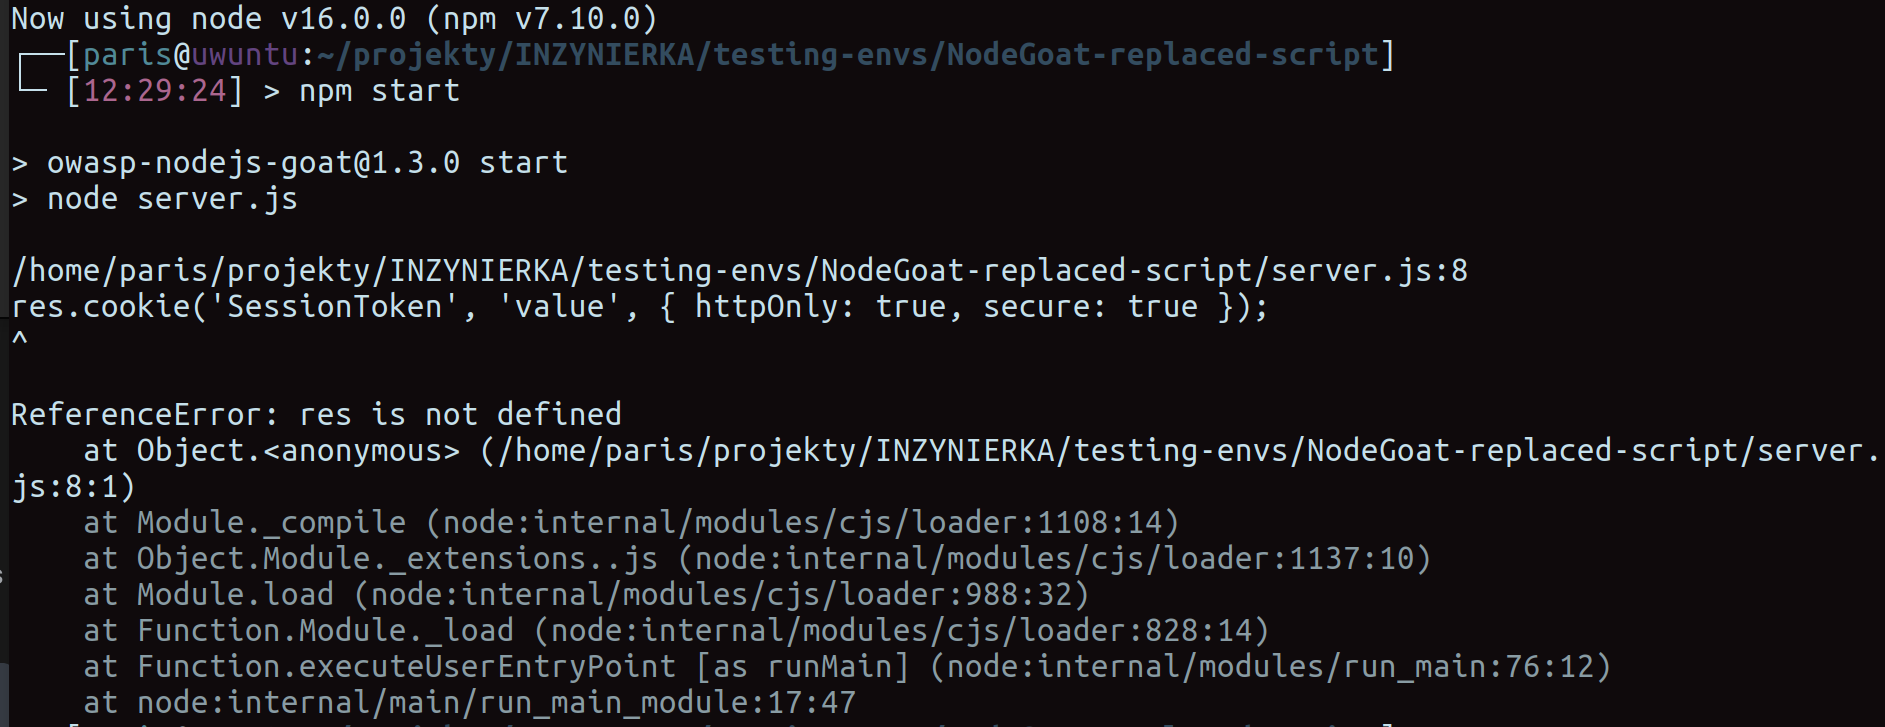
\includegraphics[width=\linewidth]{img/npm-start-error.png}
  \caption{Błąd uruchomienia aplikacji NodeGoat po wprowadzeniu zmian}
  \label{fig:nodegoat-error-after}
\end{figure}

Przykład pokazuje jak ważne jest, aby zawsze sprawdzić wyjście wygenerowane przez Szcztuczną Inteligencję, ponieważ są to algorytmy niedetermistyczne, co oznacza, że nie można przewidzieć dokładnie jakie będzie wyjście programu dla danego wejścia. W tym przypadku, program wygenerował kod, który nie był w pełni funkcjonalny, co uniemożliwiło uruchomienie aplikacji. Zaawansowane metody wprowadzania zmian w bazie kodu wejściowego przewidziane w dalszych pracach nad projektem ułatwią proces scalania kodu oraz umożliwią łatwą weryfikację wyników.

\subsection{Wprowadzenie zmian ręcznie}
Aby uniknąć konfliktów i zamieniania plików nie posiadających pełnego kodu, zdecydowałem się na ręczne wprowadzenie zmian. W tym celu skopiowałem pliki z nowej wersji do katalogu z aplikacją NodeGoat, uważnie sprawdzając ich treść i ręcznie łącząc kod. Niestety wiele zmian było gruntownych wymagających generowania certyfikatów, implementacji systemów hashujących i tym podobnych co utrudnia wprowadzenie zmian w krótkim czasie.

Następnie uruchomiłem aplikację i sprawdziłem czy działa poprawnie. Po uruchomieniu aplikacji, przeprowadziłem testy funkcjonalne, które potwierdziły poprawność działania aplikacji. 

\begin{figure}[H]
  \centering
  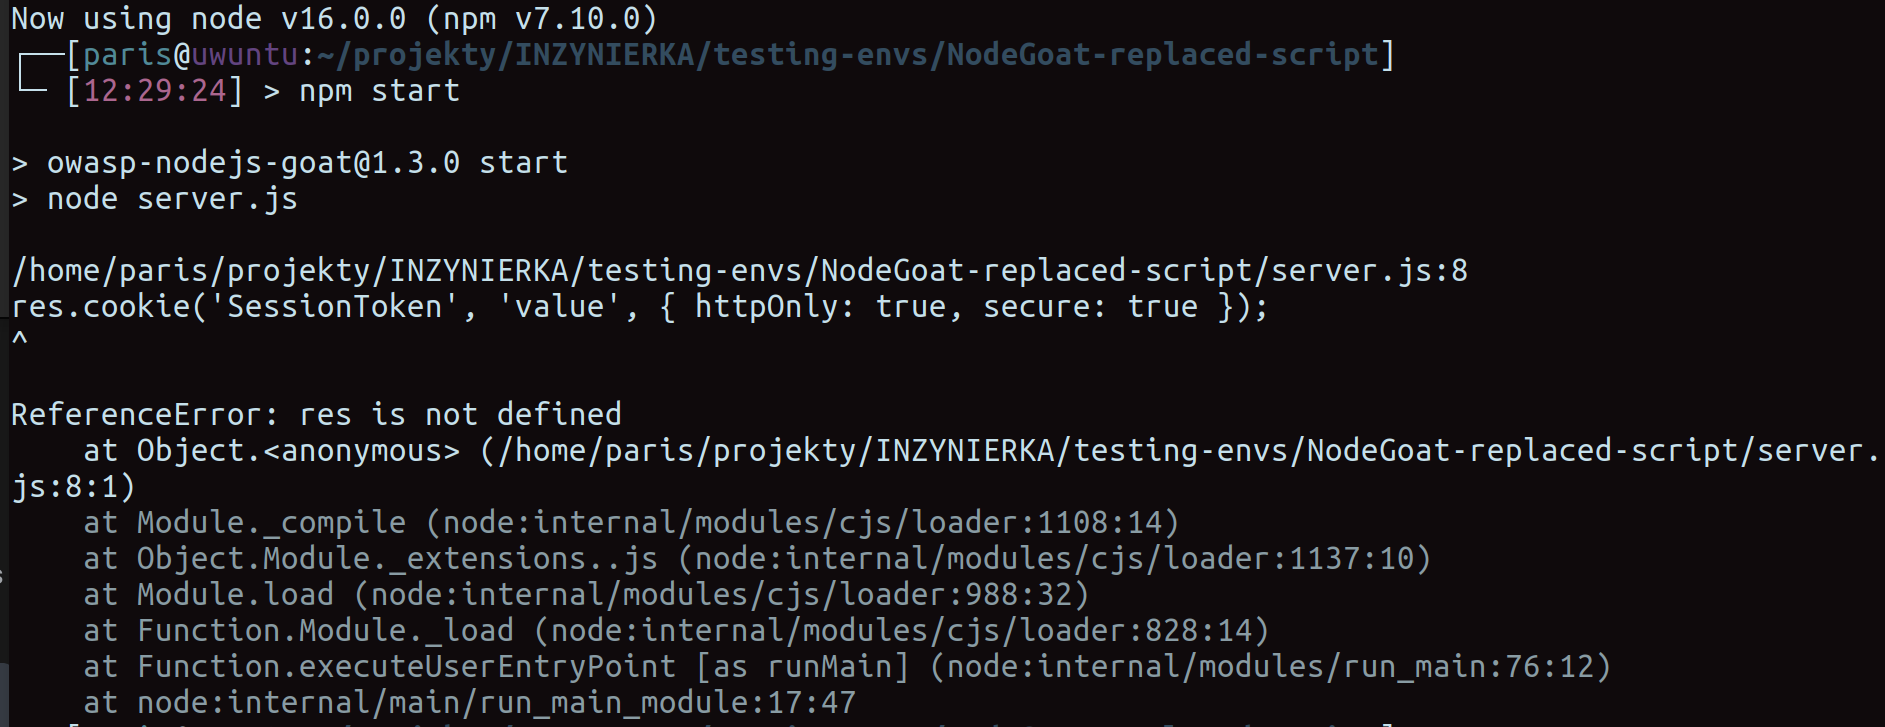
\includegraphics[width=\linewidth]{img/npm-start-error.png}
  \caption{Błąd uruchomienia aplikacji NodeGoat po wprowadzeniu zmian ręcznie}
  \label{fig:nodegoat-error-manual}
\end{figure}

Błąd wystąpił w pliku, w którym błędnie złączyłem kod. Do naprawy użyłem wersji przeglądarkowej ChatGPT, która znalazła błąd i podpowiedziała jak go naprawić. Po naprawie błędu, należało skonfigurować bazę danych MongoDB, tak by używała certyfikatów.

\begin{figure}[H]
  \centering
  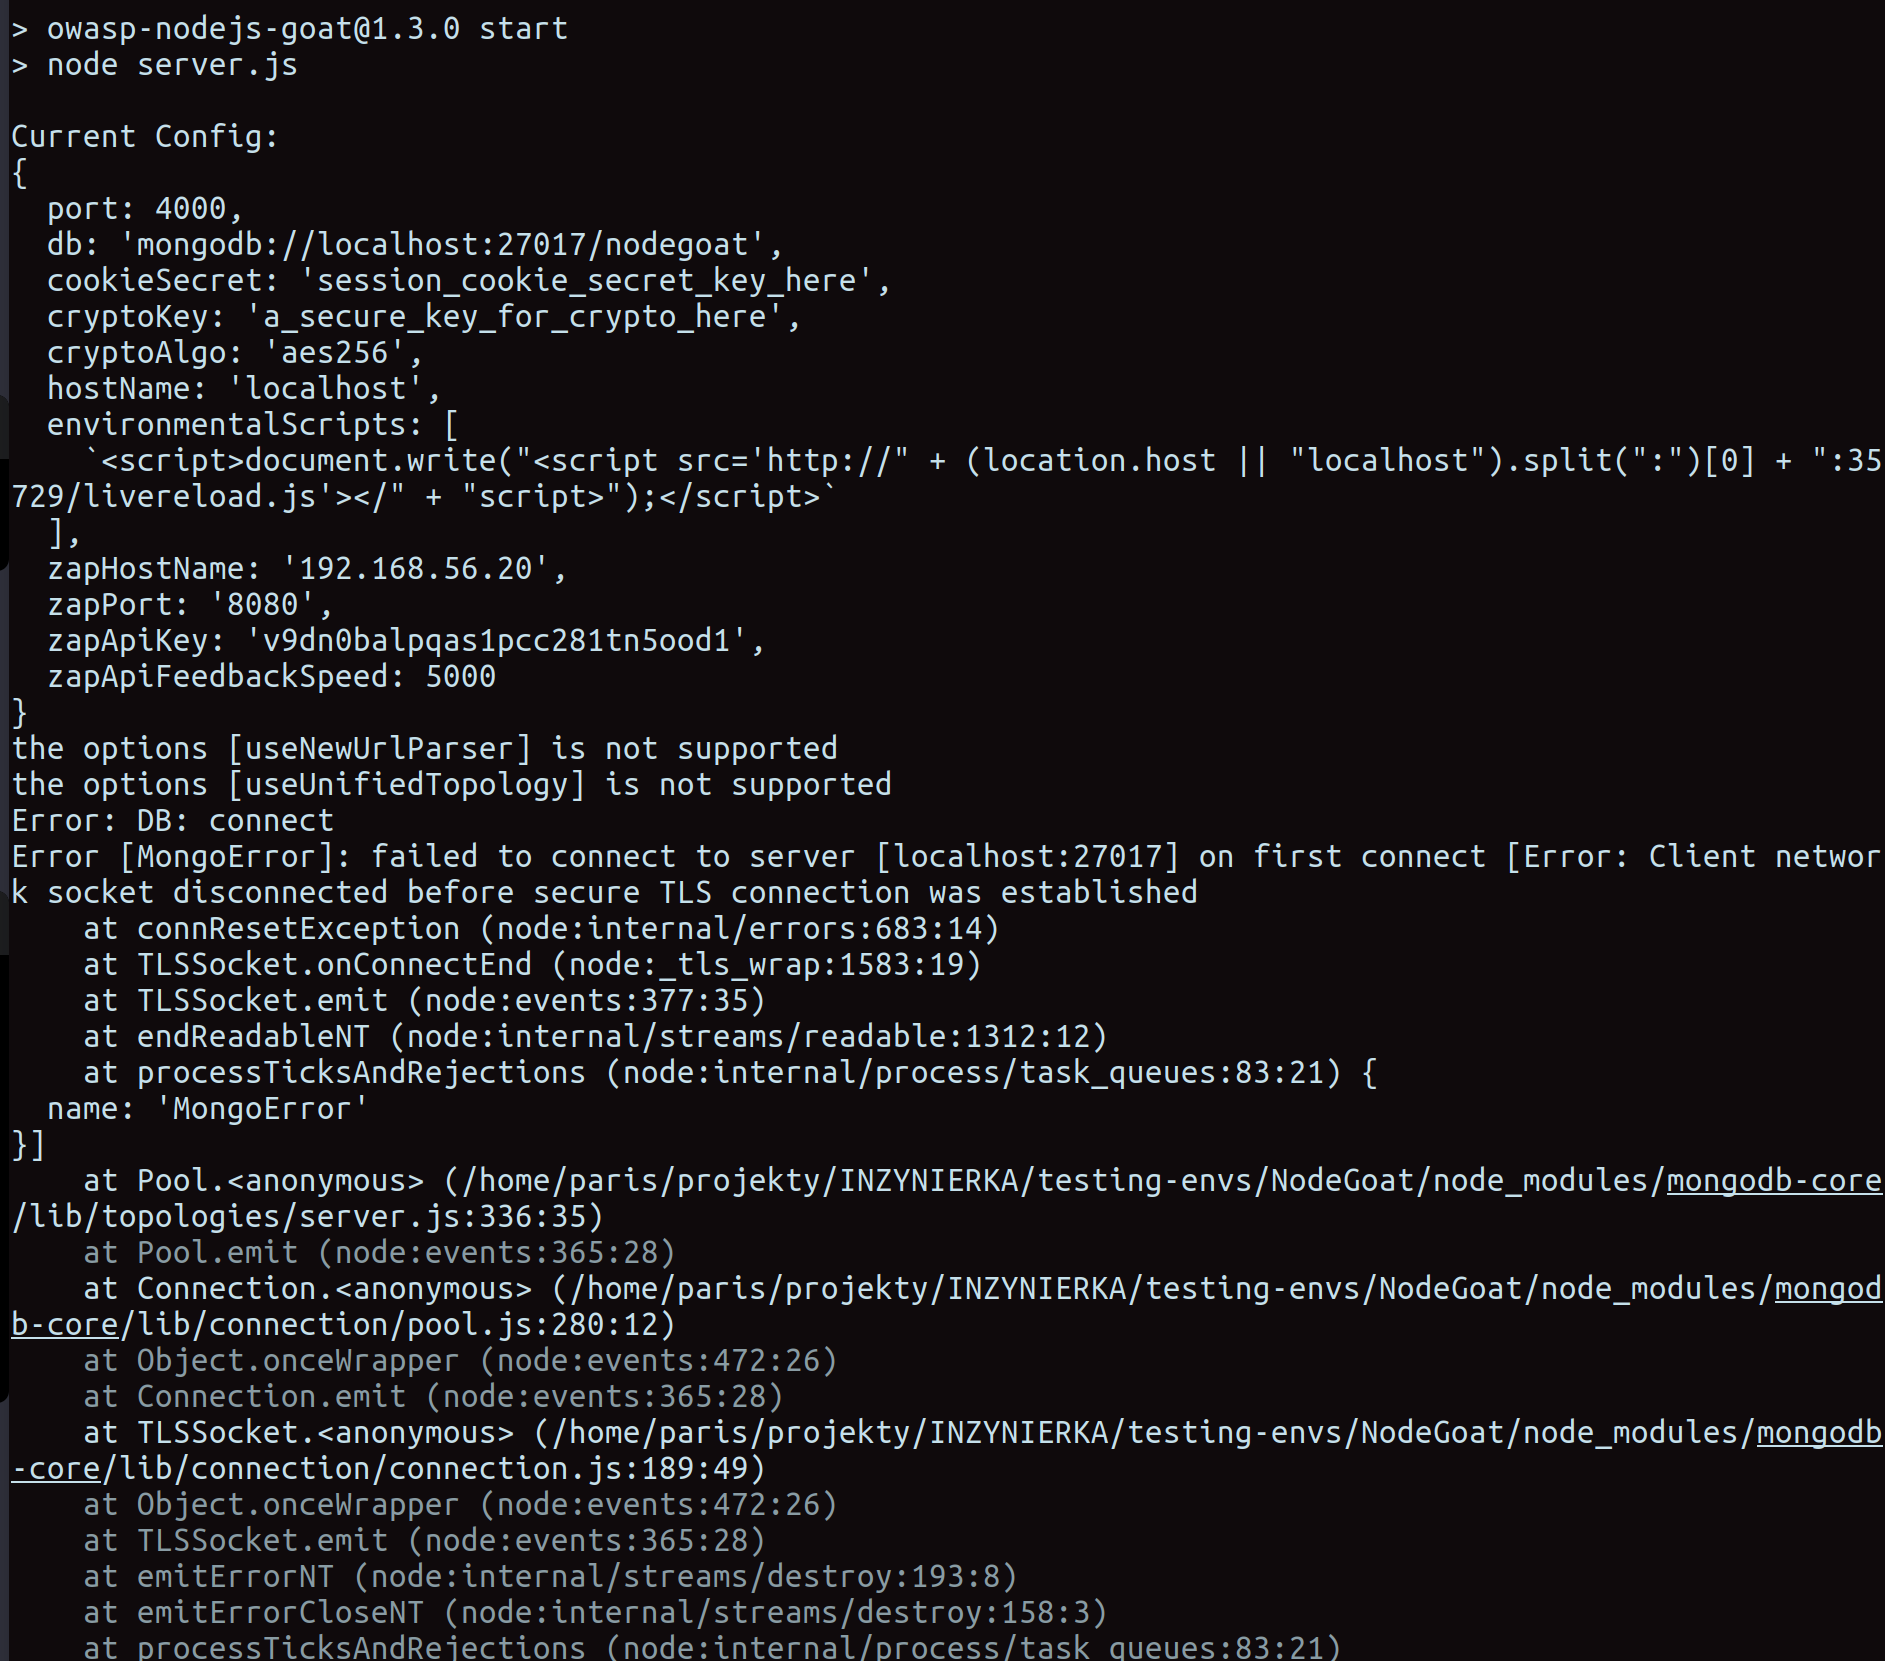
\includegraphics[width=\linewidth]{img/mongod-cert.png}
  \caption{Błąd konfiguracji MongoDB po wprowadzeniu zmian ręcznie}
  \label{fig:mongod-error}
\end{figure}

Po aktualizacji konfiguracji, aplikacja uruchomiła się poprawnie. Następnie przeprowadziłem testy funkcjonalne, które potwierdziły poprawność działania aplikacji.

\begin{figure}[H]
  \centering
  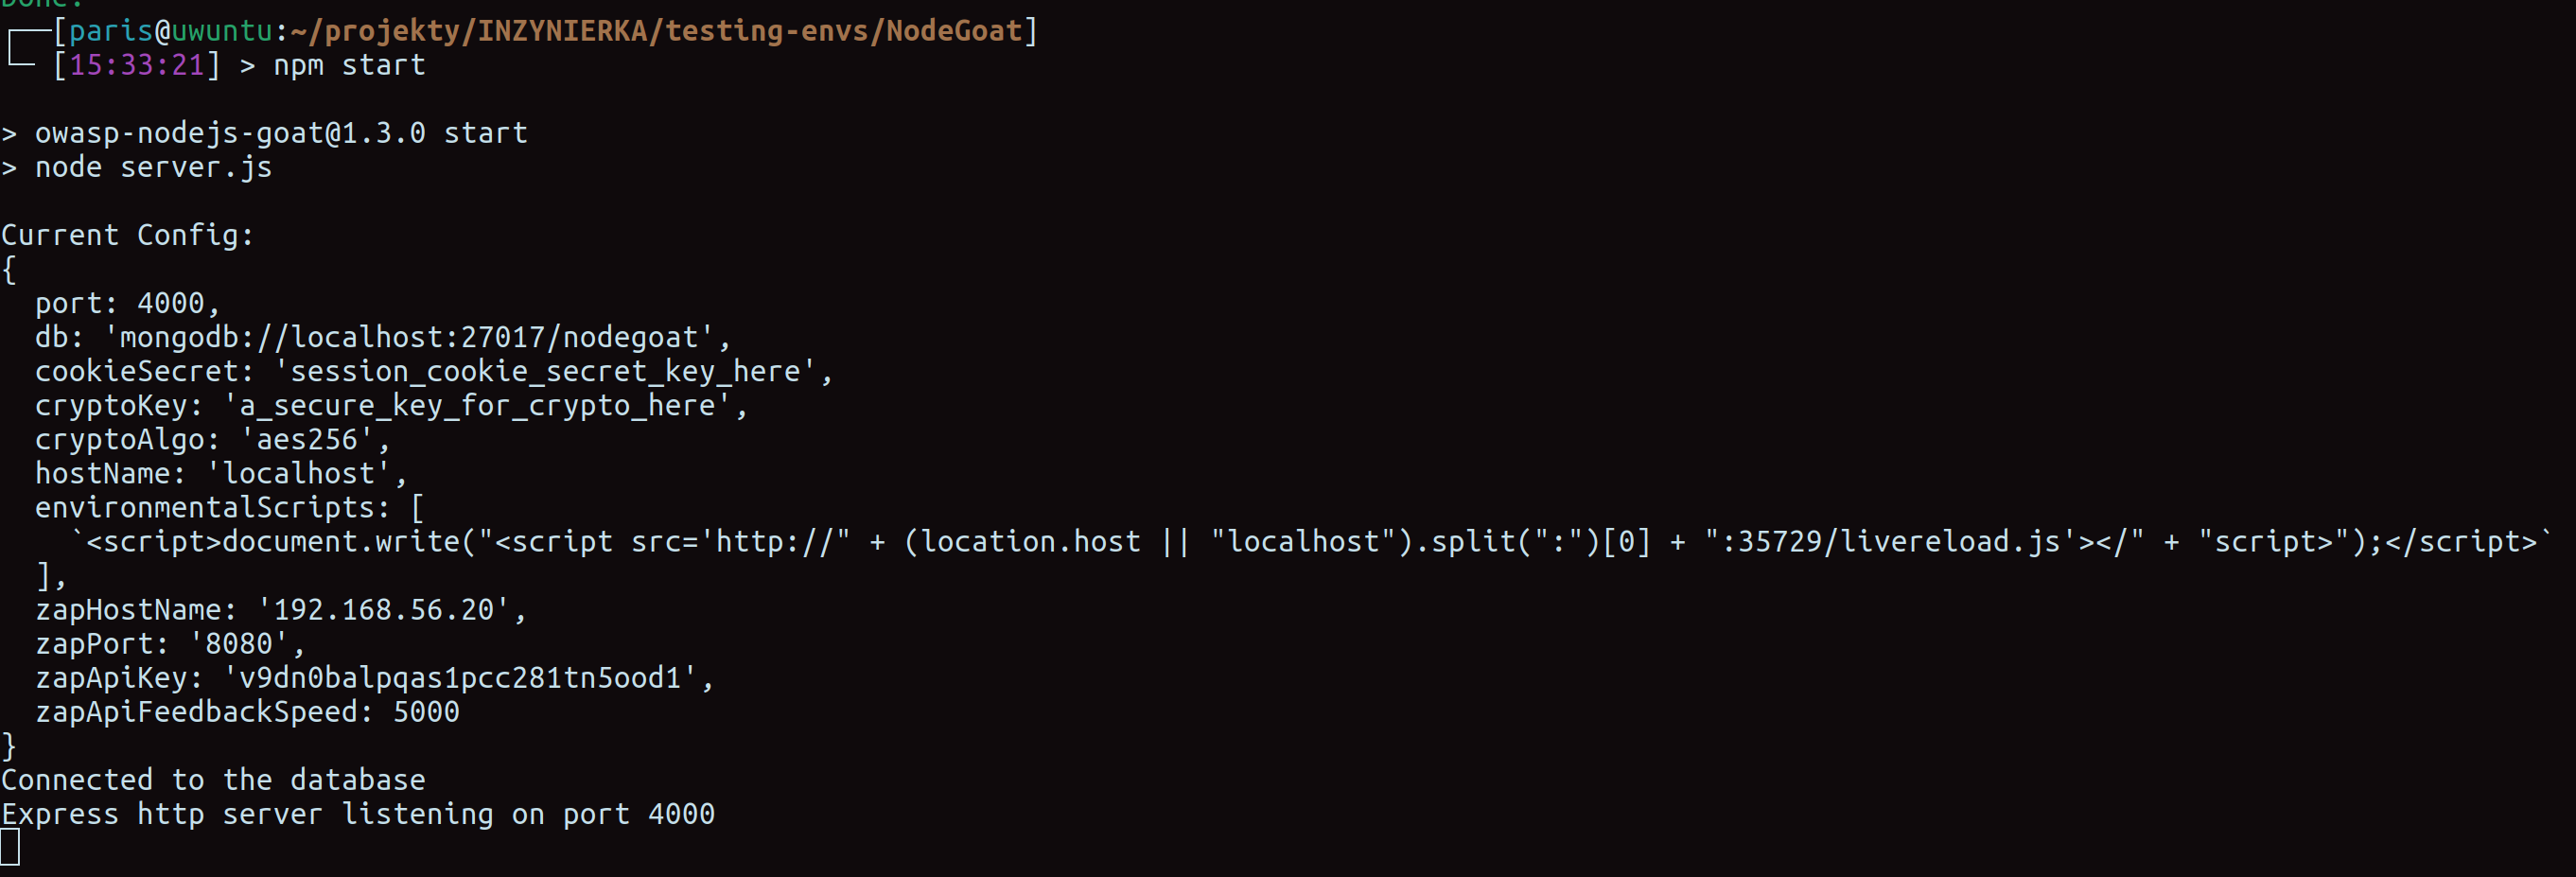
\includegraphics[width=\linewidth]{img/npm-start-success.png}
  \caption{Poprawne uruchomienie aplikacji NodeGoat po wprowadzeniu zmian ręcznie}
  \label{fig:nodegoat-success-manual}
\end{figure}

\subsection{Testy funkcjonalne po wprowadzeniu zmian}
\begin{table}[H]
  \centering
  \caption{Wyniki testów funkcjonalnych aplikacji NodeGoat po wprowadzeniu zmian ręcznie}
  \label{table:test_results}
  \begin{tabular}{|l|l|l|l|l|l|}
  \hline
  \textbf{Spec} & \textbf{Time} & \textbf{Tests} & \textbf{Passing} & \textbf{Failing} & \textbf{Skipped} \\ \hline
  allocations\_spec.js & 00:10 & 4 & 1 & 1 & 2 \\ \hline
  benefits\_spec.js & 00:02 & 5 & - & 1 & 4 \\ \hline
  contributions\_spec.js & 00:02 & 4 & - & 1 & 3 \\ \hline
  dashboard\_spec.js & 00:01 & 4 & - & 1 & 3 \\ \hline
  general\_spec.js & 00:01 & 3 & - & 1 & 2 \\ \hline
  learn\_spec.js & 00:01 & 2 & - & 1 & 1 \\ \hline
  login\_spec.js & 00:02 & 8 & - & 1 & 7 \\ \hline
  logout\_spec.js & 00:03 & 3 & - & 3 & - \\ \hline
  memos\_spec.js & 00:02 & 4 & - & 1 & 3 \\ \hline
  profile\_spec.js & 00:02 & 5 & - & 1 & 4 \\ \hline
  research\_spec.js & 00:01 & 4 & - & 1 & 3 \\ \hline
  signup\_spec.js & 00:02 & 5 & - & 1 & 4 \\ \hline
  tutorial\_spec.js & 00:08 & 13 & - & 13 & - \\ \hline
  \multicolumn{2}{|r|}{\textbf{Total (13 of 13 failed)}} & 64 & 1 & 27 & 36 \\ \hline
  \end{tabular}
  \end{table}
\normalsize

Niestety konfiguracje nadal nie były poprawne, a w plikach znajdowały się błędy typu not defined. W związku z tym, należało ręcznie wprowadzić zmiany w plikach konfiguracyjnych i zdebugować aplikację (przede wszystkim poprawne definicje zewnętrznych bibliotek oraz użycie mongodb zgodnie z dokumentacją nowej wersji sterownika). Problemem była również implementacja funkcji skrótu mających na celu umieszczanie bezpieczne przechowywanie haseł w bazie danych. Po wprowadzeniu zmian, aplikacja uruchomiła się. Następnie przeprowadziłem testy funkcjonalne, które wykazały wiele błędów aplikacji.

\begin{table}[H]
  \centering
  \caption{Test Results Summary}
  \label{table:test_results_summary}
  \begin{tabular}{|l|l|l|l|l|}
  \hline
  \textbf{Spec} & \textbf{Time} & \textbf{Tests} & \textbf{Passing} & \textbf{Failing} \\ \hline
  allocations\_spec.js & 00:18 & 4 & 1 & 3 \\ \hline
  benefits\_spec.js & 00:22 & 5 & 1 & 4 \\ \hline
  contributions\_spec.js & 00:17 & 4 & 1 & 3 \\ \hline
  dashboard\_spec.js & 00:15 & 4 & 1 & 3 \\ \hline
  general\_spec.js & 00:10 & 3 & 1 & 2 \\ \hline
  learn\_spec.js & 00:05 & 2 & 1 & 1 \\ \hline
  login\_spec.js & 00:19 & 8 & 5 & 3 \\ \hline
  logout\_spec.js & 00:04 & 3 & 3 & 0 \\ \hline
  memos\_spec.js & 00:17 & 4 & 1 & 3 \\ \hline
  profile\_spec.js & 00:18 & 5 & 2 & 3 \\ \hline
  research\_spec.js & 00:11 & 4 & 1 & 3 \\ \hline
  signup\_spec.js & 00:13 & 5 & 3 & 2 \\ \hline
  tutorial\_spec.js & 00:05 & 13 & 13 & 0 \\ \hline
  \multicolumn{2}{|r|}{\textbf{Total (11 of 13 failed)}} & 64 & 34 & 30 \\ \hline
  \end{tabular}
  \end{table}

Problematyczna okazała się implementacja porównania haseł w pliku \texttt{user-dao.js}. W nowej wersji aplikacji, hasła były zapisywane w bazie danych w postaci hashu, co wymagało zmiany sposobu porównywania haseł. Błędy mogły wynikać z różnych sposobów implementacji tych funkcji kryptograficznych w różnych plikach, które wynikały z podzielenia projektu do analizy na części.

\subsection{Testy bezpieczeństwa po wpowadzeniu zmian}
Po wprowadzeniu zmian, przeprowadziłem testy bezpieczeństwa aplikacji. W tym celu wykorzystałem narzędzie OWASP ZAP, które pozwala na przeprowadzenie testów bezpieczeństwa aplikacji internetowych. 
      \subsubsection*{OWASP ZAP}
\begin{table}[H]
  \caption{Wyniki skanowania aplikacji NodeGoat przy użyciu skanera \texttt{OWASP-zap}}
  \begin{tabular}{llllll}
    \multicolumn{2}{l}{} &
      \multicolumn{4}{c}{Risk} \\ \cline{3-6} 
    \multicolumn{2}{l|}{} &
      \multicolumn{1}{l|}{\begin{tabular}[c]{@{}l@{}}High\\ (= High)\end{tabular}} &
      \multicolumn{1}{l|}{\begin{tabular}[c]{@{}l@{}}Medium\\ (\textgreater{}= Medium)\end{tabular}} &
      \multicolumn{1}{l|}{\begin{tabular}[c]{@{}l@{}}Low\\ (\textgreater{}= Low)\end{tabular}} &
      \multicolumn{1}{l|}{\begin{tabular}[c]{@{}l@{}}Informational\\ (\textgreater{}= Informational)\end{tabular}} \\ \cline{2-6} 
    \multicolumn{1}{l|}{site} &
      \multicolumn{1}{l|}{http://localhost:4000} &
      \multicolumn{1}{l|}{\begin{tabular}[c]{@{}l@{}}0\\ (0)\end{tabular}} &
      \multicolumn{1}{l|}{\begin{tabular}[c]{@{}l@{}}5\\ (5)\end{tabular}} &
      \multicolumn{1}{l|}{\begin{tabular}[c]{@{}l@{}}3\\ (8)\end{tabular}} &
      \multicolumn{1}{l|}{\begin{tabular}[c]{@{}l@{}}5\\ (13)\end{tabular}} \\ \cline{2-6} 
    \end{tabular}   
  \label{tab:zap_after}
  \end{table}

  OWASP ZAP wykrył 13 podatności, w tym 5 o średnim ryzyku, 3 o niskim ryzyku i 5 informacyjnych. Wśród nich były podatności takie jak:
  \begin{table}[H]
    \centering
    \caption{Summary of Security Alert Types, Risks, and Counts}
    \label{tab:security_alerts}
    \begin{adjustwidth}
    {-1cm}{}
    \footnotesize
    \begin{tabular}{|l|l|l|}
      \hline
      \textbf{Alert Type} & \textbf{Risk Level} & \textbf{Count (\%)} \\
      \hline
      CSP: Wildcard Directive & Medium & 16 (123.1\%) \\
      Content Security Policy (CSP) Header Not Set & Medium & 18 (138.5\%) \\
      Directory Browsing & Medium & 2 (15.4\%) \\
      Missing Anti-clickjacking Header & Medium & 18 (138.5\%) \\
      Vulnerable JS Library & Medium & 2 (15.4\%) \\
      Server Leaks Information via "X-Powered-By" HTTP Response Header Field(s) & Low & 45 (346.2\%) \\
      Timestamp Disclosure - Unix & Low & 1 (7.7\%) \\
      X-Content-Type-Options Header Missing & Low & 25 (192.3\%) \\
      Authentication Request Identified & Informational & 1 (7.7\%) \\
      Information Disclosure - Suspicious Comments & Informational & 16 (123.1\%) \\
      Modern Web Application & Informational & 16 (123.1\%) \\
      User Agent Fuzzer & Informational & 120 (923.1\%) \\
      User Controllable HTML Element Attribute (Potential XSS) & Informational & 13 (100.0\%) \\
      \hline
    \end{tabular}
  \end{adjustwidth}
    \end{table}

    \subsubsection*{CodeQL}
    \begin{table}[H]
      \centering
      \caption{Streszczone wyniki skanowania aplikacji NodeGoat przy użyciu skanera \texttt{CodeQL}}
      \label{table:security_issues}
      \resizebox{\textwidth}{!}{%
      \begin{tabular}{|p{0.20\linewidth}|p{0.40\linewidth}|p{0.10\linewidth}|p{0.15\linewidth}|p{0.15\linewidth}|}
      \hline
      \textbf{Issue} & \textbf{Description} & \textbf{Level} & \textbf{File} & \textbf{Occurrences} \\ \hline
      Polynomial regular expression & Vulnerable to DoS attacks. Slow on strings with many '0' repetitions or starting with '\t@'. & Warning & profile.js, session.js & 2 \\ \hline
      Clear-text logging of sensitive info & Exposes sensitive data like passwords to attackers. & Error & user-dao.js & Multiple \\ \hline
      Database query from user input & Vulnerable to code injection by the user. & Error & user-dao.js & 2 \\ \hline
      Missing CSRF middleware & Lack of CSRF protection can allow malicious request submissions. & Error & server.js & Multiple \\ \hline
      Rate limiting & Lack of rate limiting can lead to DoS attacks. & Warning & index.js & 1 \\ \hline
      Server-side request forgery & Network requests with user data in URL can allow for attacks. & Error & research.js & 1 \\ \hline
      DOM text as HTML & Can lead to cross-site scripting vulnerabilities. & Warning & bootstrap.js & Multiple \\ \hline
      Unsafe jQuery plugin & Constructs HTML from options, potential XSS vulnerability. & Warning & bootstrap.js & Multiple \\
      \hline
      \end{tabular}%
      }
      \end{table}
      

    Po przeprowadzeniu popraw wykrytych zostało mniej podatności, co udowadnia o zwiększeniu bezpieczeństwa, dzięki wprowadzonym zmianom. Niestety zmiany te sprawiają, że aplikacja nie jest w pełni funkcjonalna, co może się przyczyniać do lepszych wyników skanu bezpieczeństwa.

\section{Identyfikacja podatności bez podpowiedzi w kodzie}
W kodzie aplikacji NodeGoat znajdowało się wiele wskazówek dotyczących podatności. Znacznie to ułatwia proces analizy kodu dla dużych modeli językowych, ponieważ mogę skupić się na konkretnych, wskazanych fragmentach kodu. W celu sprawdzenia jakie podatności wykryje GPTester bez podpowiedzi w kodzie, przeprowadziłem analizę kodu aplikacji NodeGoat bez podpowiedzi w kodzie. \\

{\large\textbf{Wyniki analizy kodu aplikacji NodeGoat bez podpowiedzi w kodzie}}
\normalsize
\begin{enumerate}
    \item \textbf{MongoClient Connection String Exposure}: The \texttt{db} variable likely contains the connection string to MongoDB, which includes credentials. This sensitive information can be exposed if the configuration file is not properly secured.
    \item \textbf{Insecure Express Session Configuration}: The session middleware in \texttt{server.js} uses a cookieSecret from a config file for signing cookies, but it does not have secure attributes such as \texttt{httpOnly}, \texttt{secure}, \texttt{sameSite}, as well as not using a store which can lead to security issues.
    \item \textbf{SWIG Template Auto-Escape Disabled}: In \texttt{server.js}, the SWIG template engine is used with \texttt{autoescape: false}, making it vulnerable to Cross-Site Scripting (XSS) attacks if user input is included in templates.
    \item \textbf{Use of Marked Library for Markdown Parsing}: The marked library is being used in \texttt{server.js} with the \texttt{sanitize} option set to \texttt{true}, which is good for preventing XSS. However, if library updates change the default behavior, it could lead to vulnerabilities.
    \item \textbf{Database Reset Script}: In \texttt{db-reset.js}, the process exits with a different status code in case of an error. This can lead to inconsistent behavior and potentially leak information about the database status or structure.
    \item \textbf{Lack of HTTPS}: The server in \texttt{server.js} is started with HTTP and not HTTPS, leading to the exposure of data in transit.
    \item \textbf{Open Docker Ports in Development}: The \texttt{docker-compose.yml} file shows ports open which should not be exposed in a production environment.
    \item \textbf{Hardcoded Credentials in \texttt{db-reset.js}}: Usernames and passwords are hardcoded in the \texttt{db-reset.js} script, which is a bad practice for managing credentials.
    \item \textbf{Insecure Password Storage (user-dao.js)}: Passwords should not be stored in plaintext. The \texttt{addUser} method currently stores the password received from the user directly into the database.
    \item \textbf{Insecure Password Verification (user-dao.js)}: The \texttt{validateLogin} method uses a simple string comparison to validate passwords, which would only be secure if the passwords were properly hashed and salted before storage and then compared using a secure function.
    \item \textbf{Potential NoSQL Injection (research-dao.js, getBySymbol)}: The \texttt{getBySymbol} method creates a query without proper sanitation or parameterized queries, which may open up the application to NoSQL injection attacks.
    \item \textbf{Potential NoSQL Injection (profile-dao.js, updateUser)}: The \texttt{updateUser} method directly uses the incoming parameter \texttt{userId} after parsing it as an integer. Although this reduces the risk, it's still a good habit to use a parameterized query.
    \item \textbf{Lack of Input Validation}: Across various DAO functions, there is a lack of input validation to ensure that the values passed to the database operations do not contain malicious input.
    \item \textbf{NoSQL Injection in Allocations (allocations-dao.js)}: The method \texttt{getByUserIdAndThreshold} is susceptible to NoSQL injection as it constructs a query using a \texttt{\$where} operator with user input, which can be manipulated.
    \item \textbf{Insecure Configuration in Github Workflow (e2e-test.yml)}: The configuration file uses hardcoded version \texttt{"4.0"} for the MongoDB Docker image, which might be outdated and contain known vulnerabilities.
    \item \textbf{Arbitrary Redirect in Index Route (index.js)}: The \texttt{/learn} route redirects to a user-specified URL without validation, which can be exploited for phishing attacks.
    \item \textbf{Insufficient Logging and Monitoring in Error Handler (error.js)}: The error handling middleware logs the error message but doesn't notify the team or use a centralized logging system.
    \item \textbf{Cross-Site Scripting (XSS) in Profile Data Rendering (profile.js)}: Directly embedding user input from \texttt{doc.website} in the HTML without encoding it, which can lead to Cross-Site Scripting attacks.
    \item \textbf{Insufficient Password Strength Validation (session.js)}: The \texttt{PASS\_RE} regex allows for weak passwords that do not require a mix of character types.
    \item \textbf{Remote Code Execution in Config File (config.js)}: User input (\texttt{finalEnv}) is used to construct a file path without proper validation, which could allow an attacker to traverse the filesystem or execute arbitrary code.
    \item \textbf{Insecure Direct Object References (IDOR) in Allocations (allocations.js)}: User input from \texttt{req.params.userId} is used directly to query the database, which could allow an unauthorized user to access other users' data.
    \item \textbf{Server-Side Request Forgery (SSRF) in Research (research.js)}: The \texttt{url} and \texttt{symbol} parameters from user input are concatenated and used in a GET request without validation, allowing SSRF attacks.
    \item \textbf{Cross-Site Scripting (XSS) in Memos (memos.js)}: User input \texttt{req.body.memo} is directly inserted into the database and later rendered without proper encoding.
    \item \textbf{Command Injection in Contributions (contributions.js)}: Use of \texttt{eval} with user input \texttt{req.body.preTax}, \texttt{req.body.afterTax}, and \texttt{req.body.roth}, enabling command injection attacks.
\end{enumerate}

Wyniki pokazują, że nawet bez podpowiedzi w kodzie, GPTester jest w stanie wykryć podatności w kodzie aplikacji NodeGoat. Są to bardzo zbliżone wyniki do tych otrzymanych z podpowiedziami.  

\section{Wnioski z analizy NodeGoat}
\label{sec:wnioski}

Na podstawie przeprowadzonych testów na aplikacji NodeGoat przy użyciu GPTester oraz technik LLM można wyciągnąć następujące wnioski:

\begin{enumerate}
    \item \textbf{Potencjał LLM w identyfikacji podatności:} Large Language Models, takie jak GPT-4 wykorzystany w GPTester, wykazują potencjał w identyfikacji podatności w kodzie aplikacji. Ich zdolność do rozumienia i analizy kodu pozwala na efektywne wyszukiwanie zagrożeń bezpieczeństwa. Niestety wyniki trzeba zaktualizować o badania kodu nie posiadającego podpowiedzi, których NodeGoat posiada wiele. 
    
    \item \textbf{Ograniczenia LLM w kontekście analizy bezpieczeństwa:} Pomimo zaawansowanych możliwości, LLM napotykają ograniczenia związane z rozmiarem kodu, który mogą przetworzyć, oraz z interpretacją skomplikowanych zależności w aplikacjach. Wymaga to od programistów i specjalistów ds. bezpieczeństwa uzupełnienia analizy o ekspertyzę ludzką.
    
    \item \textbf{Znaczenie interakcji człowieka z LLM:} Wyniki generowane przez GPTester i inne narzędzia wykorzystujące LLM mogą wymagać weryfikacji i doprecyzowania przez ludzi. Skuteczność LLM w analizie podatności wzrasta przy ścisłej współpracy z ekspertami ds. bezpieczeństwa.
    
    \item \textbf{Koszty i ograniczenia zasobów:} Wykorzystanie LLM, zwłaszcza w dużych projektach, może być związane z wysokimi kosztami i ograniczeniami zasobów (np. limitami API). Optymalizacja procesu analizy pod kątem wyboru kodu do skanowania jest kluczowa dla zarządzania kosztami i efektywnością.
    
    \item \textbf{Potrzeba integracji z innymi narzędziami:} Aby uzyskać kompleksowy obraz bezpieczeństwa aplikacji, zaleca się integrację LLM z tradycyjnymi narzędziami do skanowania podatności, takimi jak OWASP ZAP czy Nessus. Takie połączenie pozwala na bardziej wszechstronną analizę.
    
    \item \textbf{Dynamika rozwoju LLM:} Szybki rozwój technologii LLM wskazuje na możliwość dalszego zwiększania ich skuteczności w analizie bezpieczeństwa aplikacji. Potencjał wykazuje również rozszerzenie parametrów dla OpenAI Assistant API. Kontynuacja badań i eksperymentów w tym obszarze jest zatem istotna.
\end{enumerate}